%!TEX root = ../aluno.tex

\ifnum\aluno=1
\renewcommand\chapterillustration{abertura-tales}
\else
\renewcommand\chapterillustration{abertura-tales-professor}
\fi
\renewcommand\chapterwhat{São estudados o significado de um teorema
com sua hipótese e tese, o Teorema de Tales, sua recíproca, as projeções paralelas e aplicações.}
\renewcommand\chapterbecause{O capítulo contém uma ferramenta útil para resolver situações que envolvem retas paralelas. Além disso, o teorema de Tales será usado para para desenvolver o conceito de semelhança de triângulos, que é um dos instrumentos necessários para compreender o mundo real. A semelhança, por sua vez, permite a obtenção de diversas propriedades métricas das figuras geométricas, tanto planas como espaciais.}


\chapter{Teorema de Tales}



\mbox{}\thispagestyle{empty}\clearpage

\thispagestyle{empty}

\begin{center}
Projeto: LIVRO ABERTO DE MATEMÁTICA

\noindent \begin{tabular}{lcccr}

\includegraphics[scale=.15]{impa}& \quad\quad& 
\includegraphics[width=3cm]{logo} & \quad\quad& 
\includegraphics[scale=.24]{obmep} 
\end{tabular}
\end{center}

\vspace*{.3cm}

Cadastre-se como colaborador no site do projeto: \url{umlivroaberto.org}

Versão digital do capítulo:

\url{https://www.umlivroaberto.org/BookCloud/Volume_1/master/view/GE201.html}

% \begin{center}
%   \includegraphics[width=2cm]{canvas}
% \end{center}

\begin{tabular}{p{.15\textwidth}p{.7\textwidth}}
Título: & Teorema de Tales\\
\\
Ano/ Versão: & 2021 / versão 1.0 de \today\\
\\
Editora & Instituto Nacional de Matem\'atica Pura e Aplicada (IMPA-OS)\\
\\
Realização:& Olimp\'iada Brasileira de Matem\'atica das Escolas P\'ublicas (OBMEP)\\
\\
Produção:& Associação Livro Aberto\\
\\
Coordenação: & Fabio Simas e Augusto Teixeira (livroaberto@impa.br)\\
\\
  Autores: & Eduardo Wagner,\\
        & Marcos Paulo\\
\\
Revisão: &  Cydara Ripoll  \\
          &  Letícia Rangel \\
\\
Design: & Andreza Moreira (Tangentes Design) \\
\\
  % Ilustrações: & Miller  Guglielmo \\ 
% \\
Gráficos: & --- \\
\\
  Capa: & Foto de Sigmund, no Unsplash \\
        & https://unsplash.com/photos/r9PeXDCJyEw \\

\end{tabular}

\begin{figure}[b]
\begin{minipage}[l]{5cm}
\centering

{\large Licença:}

  
\includegraphics[width=3.5cm]{cc-by-sa1}
\end{minipage}\hfill
\begin{minipage}[c]{5cm}
\centering
{\large Desenvolvido por}


\includegraphics[width=2.5cm]{logo-associacao.jpg}
\end{minipage}
\begin{minipage}[r]{5cm}
\centering

{\large Patrocínio:}
  \vspace{1em}
  
\includegraphics[width=3.5cm]{itau}
\end{minipage}
\end{figure}

\mainmatter


\begin{apresentacao}{Introdução}


Durante muito tempo, a Geometria plana ficou totalmente relegada ao ensino fundamental e, consequentemente, os aspectos mais refinados da sua construção foram deixados de lado. Com a inserção de tópicos de Geometria plana pela Base Nacional Comum Curricular (BNCC) no Ensino Médio, devemos modificar nossa prática de ensino de geometria para nos adequar a  essa nova realidade.


Embora iniciemos o capítulo com uma situação concreta convidando o aluno a se familiarizar com o modelo geométrico dessa situação, temos como objetivo maior introduzir um pouco mais de rigor nos assuntos abordados neste capítulo.


\begin{habilities}{EM12MT01}

Compreender o teorema de Tales e aplicá-lo em demonstrações e na resolução de problemas, incluindo a divisão de segmentos em partes proporcionais.
\end{habilities}

Observamos que, no contexto do Ensino Médio, “Compreender o teorema de Tales” vai além da capacidade de reconhecer uma figura em que o teorema de Tales é aplicável. Esperamos que o aluno seja capaz de justificar outros teoremas a partir do teorema de Tales, como na atividadeda da seção “\DUrole{xref,std,std-ref}{sub-divisao-de-segmentos}”.

Algumas propriedades geométricas precisam estar compreendidas para que se possa demonstrar o teorema de Tales e, por isso, neste capítulo foram incluídas rápidas visitas aos temas “Retas Paralelas” e “Congruência de Triângulos”.

A demonstração inicial do teorema de Tales será feita no caso dos segmentos comensuráveis e, no final do capítulo aparecerá a demonstração geral.

Algumas recomendações:
\begin{itemize}
\item {} 
Alunos conhecem em níveis diferentes o Teorema de Tales. Procure explorar com perguntas para verificar o nível de profundidade da familiaridade de seus alunos.

\item {} 
Uma das atividades iniciais, ``\hyperref[nas-ruas]{Nas ruas de uma cidade}”, é solicitado que os alunos façam uma estimativa. Estimule estimativas sem cálculo para comparar com o resultado que posteriormente será encontrado.

\item {} 
No ensino Fundamental, a maioria das propriedades eram compreendidas através de observações das figuras. No ensino Médio entendemos que algumas demonstrações devem ser efetuadas para que o aluno perceba o aspecto construtivo da Matemática.

\item {} 
A seção Organizando as ideias: medidas de dispersão é tão importante como delicada, pois trata da metodologia de demonstração. Um dos aspectos fundamentais de separação de \textbf{Hipótese} e \textbf{Tese} deve ser incentivado. Convide, sempre que possível, seus alunos a reescrever teoremas com os quais eles já têm familiaridade usando a estrutura de “Se Hipótese, então Tese”.

\item {} 
Dentre os exercícios, é proposto um de demonstração do teorema das Bissetrizes, que decorre diretamente do teorema de Tales.

\end{itemize}

\end{apresentacao}

\cleardoublepage
\def\currentcolor{session1}


\begin{objectives}{Nas ruas de uma cidade}
{
Levar o estudante a:
\begin{itemize}
\item {} 
Reconhecer retas paralelas.

\item {} 
Estimar uma distância.

\item {} 
Praticar sua intuição

\end{itemize}
}{1}{1}
\end{objectives}
\begin{sugestions}{Nas ruas de uma cidade}
{
\begin{itemize}
\item {} 
Os valores mencionados no desenho são bem próximos dos reais.

\item {} 
No item \titem{a)}, esperamos apenas que o aluno perceba o paralelismo entre as ruas, nada mais.

\item {} 
No item b), sem cálculos, entendemos que visualmente, uma estimativa entre $180$ m e $190$ m é excelente.

\item {} 
É conveniente verificar se alguns alunos utilizaram regra de três, mostrando que já tinham trazido esse conceito do Ensino Fundamental.

\end{itemize}
}{1}{1}
\end{sugestions}
\begin{answer}{Nas ruas de uma cidade}
{
\begin{enumerate}
\item {} 
São paralelas.

\item {} 
Qualquer valor entre $180$ m e $190$ m.

\item {} 
Resposta pessoal.

\end{enumerate}
}{1}
\end{answer}
\clearmargin

\begin{objectives}{Recordando paralelas}
{
Levar o estudante a
\begin{itemize}
\item {} 
Reconhecer ângulos em paralelas cortadas por transversal.

\item {} 
Reconhecer os ângulos que são iguais nessa situação.

\item {} 
Lembrar um caso de congruência de triângulos.

\end{itemize}
}{1}{2}
\end{objectives}
\begin{sugestions}{Recordando paralelas}
{
\begin{itemize}
\item {} 
Neste texto, segmentos congruentes serão chamados de iguais. Da mesma forma, ângulos congruentes serão também chamados de iguais.

\item {} 
A relação de igualdade entre os ângulos \(a\), \(b\) e \(c\) é conhecida desde o Ensino Fundamental. No último exercício do capítulo o aluno vai usar esses fatos como argumento para demonstrar que certo triângulo é isósceles.

\item {} 
Se o aluno não conhecer os casos de congruência de triângulos, ela pode ser verificada de maneira informal a partir de sobreposição por dobradura ou recortando um desenho semelhante.

\item {} 
Para uma justificativa matemáticamente rigorosa, necessitamos dos critérios de congruência de triângulos que estarão no Organizando as ideias após a atividade.

\end{itemize}
}{1}{2}
\end{sugestions}
\begin{answer}{Recordando paralelas}
{
\begin{enumerate}
\item {} 
Alternos internos

\item {} 
São iguais

\item {} 
Correspondentes

\item {} 
São iguais.

\item {} 
Porque possuem os mesmos ângulos internos e têm o lado AC em comum.

\item {} 
São iguais. São iguais também

\end{enumerate}
}{1}
\end{answer}




\explore{}

O teorema de Tales é um resultado básico da geometria plana e vai permitir a exploração e dedução de outros resultados, também centrais, dessa matéria. O teorema de Tales (das retas paralelas) é conhecido desde a antiguidade. Tales de Mileto viveu no século 6 a.C., mas nenhum dos seus escritos sobreviveu. Tudo o que sabemos dele veio através de escritos de outros.

\begin{task}{Nas ruas de uma cidade}
\label{nas-ruas}



A figura a seguir mostra uma parte da cidade de Nova York. Nessa região, as ruas são designadas por números. Observe as ruas numeradas de 67 a 71, as Avenidas Columbus e Broadway.

\begin{figure}[H]
\centering

\noindent\includegraphics[width=200bp]{{Fig-tales-01}.png}
\end{figure}

A distância \(A\) entre duas esquinas consecutivas da Avenida Columbus é igual a \(70\) m e a distância \(B\) entre as respectivas esquinas correspondentes na Broadway é \(80\) m. A distância \(C\) entre as esquinas da Columbus com as ruas 69 e 71 é  \(161\) m, e a distância entre as esquinas correspondentes na Broadway é \(D\).
\begin{enumerate}
\item {} 
Você lembra quais são as possíveis posições relativas entre duas retas no plano? Que relação você vê entre as ruas de 67 a 71?

\item {} 
Visualmente, estime um valor para a distância \(D\).

\item {} 
Você consegue calcular a distância \(D\)?

\end{enumerate}
\end{task}


\begin{task}{Recordando paralelas}



Na figura a seguir estão representados dois pares de retas paralelas: o par de retas \(AD\) e \(BC\) e o par de retas \(AB\) e \(CD\).
\begin{center}\begin{tikzpicture}
legenda
\draw [shift={(-0.7404492822759008,2.0323275076976457)},line width=0.8pt,color=session2,fill=session2,fill opacity=0.10000000149011612] (0,0) -- (-158.99677728856574:0.40327274248797285) arc (-158.99677728856574:-103.61977057805956:0.40327274248797285) -- cycle;
\draw [shift={(-1.2241649681252438,0.03590094973762964)},line width=0.8pt,color=session2,fill=session2,fill opacity=0.10000000149011612] (0,0) -- (21.003222711434265:0.40327274248797285) arc (21.003222711434265:76.38022942194044:0.40327274248797285) -- cycle;
\draw [shift={(2.5915772583373085,1.500873411683074)},line width=0.8pt,color=session2,fill=session2,fill opacity=0.10000000149011612] (0,0) -- (21.003222711434265:0.40327274248797285) arc (21.003222711434265:76.38022942194043:0.40327274248797285) -- cycle;
\draw [line width=0.8pt] (-2.62,-0.5)-- (4.1,2.08);
\draw [line width=0.8pt] (-2.7,1.28)-- (4.0347849649135,3.8656763704578623);
\draw [line width=0.8pt] (-1.48,-1.02)-- (-0.38,3.52);
\draw [line width=0.8pt] (2.32,0.38)-- (3.313758477838472,4.481512263078785);
\draw [line width=0.8pt] (-0.7404492822759008,2.0323275076976457)-- (2.5915772583373085,1.500873411683074);
\draw (-1.2,2.6) node[anchor=north west] {A};
\draw (-1.3,0) node[anchor=north west] {B};
\draw (2.5,1.4) node[anchor=north west] {C};
\draw (2.5,4) node[anchor=north west] {D};
\draw (-1.4,1.7) node[anchor=north west] {$ a $};
\draw (-1,.9) node[anchor=north west] {$ b $};
\draw (2.8,2.3) node[anchor=north west] {$ c $};
\draw [line width=2.pt,color=session3] (-1.2241649681252438,0.03590094973762964)-- (-0.7404492822759008,2.0323275076976457);
\draw [line width=2.pt,color=session3] (2.5915772583373085,1.500873411683074)-- (3.075292944186652,3.4972999696430898);
\begin{scriptsize}
\draw [fill=black] (-0.7404492822759008,2.0323275076976457) circle (1.0pt);
\draw [fill=black] (-1.2241649681252438,0.03590094973762964) circle (1.0pt);
\draw [fill=black] (2.5915772583373085,1.500873411683074) circle (1.0pt);
\draw [fill=black] (3.075292944186652,3.4972999696430898) circle (1.0pt);
\end{scriptsize}
\end{tikzpicture}\end{center}\begin{enumerate}
\item {} 
Você conhece o nome que se dá ao par de ângulos \(a\) e \(b\)?

\item {} 
Que relação há entre os ângulos \(a\) e \(b\)?

\item {} 
Você conhece o nome que se dá ao par de ângulos \(b\) e \(c\)?

\item {} 
Que relação há entre os ângulos \(b\) e \(c\)?

\item {} 
Pode-se afirmar que os triângulos \(ABC\) e \(CDA\) são congruentes. Por quê?

\item {} 
Que relação existe entre os segmentos \(AB\) e \(CD\)? E com os segmentos \(AD\) e \(BC\)?

\end{enumerate}
\end{task}


\clearpage

\arrange{}
\begin{texto}
{\def\currentcolor{session4}
\begin{observation}{}
Vale lembrar que serão utilizados conceitos do Ensino Fundamental. Em alguns casos, será necessário que se recorde tais conceitos para poder avançar no capítulo.
\begin{itemize}
\item {} 
Ângulos nas paralelas cortadas por uma transversal;

\item {} 
A definição de paralelogramo (Quadrilátero que possui dois pares de lados paralelos).

\end{itemize}
\end{observation}
}
\end{texto}
\clearmargin
\begin{objectives}{Demonstrando uma afirmação}
{
Levar o estudante a
\begin{itemize}
\item {} 
Demonstrar um resultado.

\item {} 
Identificar, em uma proposição, as hipóteses e o que se que demonstrar.

\item {} 
Planejar a sequência de argumentos para concluir o resultado.

\end{itemize}

}{1}{2}
\end{objectives}
\begin{sugestions}{Demonstrando uma afirmação}
{
\begin{itemize}
\item {} 
Essa proposição é um teorema, mas ainda não estamos dando esse título, pois não é o objetivo no momento.

\item {} 
Para demonstrar a proposição é necessário interferir na figura, traçando novos segmentos que vão permitir o aparecimento de triângulos congruentes. Nessa primeira atividade de demonstração, daremos as dicas para que o aluno consiga percorrer o caminho até o final.

\end{itemize}
}{1}{2}
\end{sugestions}
\begin{answer}{Demonstrando uma afirmação}
{
\begin{enumerate}
\item {} 
\(DE = EF\) (caso tivessesmo escolhido considerar inicialmente \(DE=EF\), a resposta seria \(AB=BC\)).

\item {} 
Os triângulos \(DGE\) e \(EHF\) são congruentes pelo caso \textbf{ALA}.

De fato, \(ABGD\) e \(BCHE\) são paralelogramos. Daí, \(DG = AB = BC = EH\).

Além disso, os dois triângulos possuem mesmos ângulos pois \(DG\) e \(EH\) são paralelos, da mesma forma que \(GE\) e \(HF\) são também paralelos.

\item {} 
Dessa congruência conclui-se que \(DE = EF\) que queríamos demonstrar

\end{enumerate}
}{1}
\end{answer}
\clearmargin
\def\currentcolor{session2}
\begin{objectives}{Dividindo um segmento em partes iguais}
{
Levar o estudante a
\begin{itemize}
\item {} 
Perceber que nossa visão é limitada e nossos instrumentos de medida são limitados e imperfeitos.

\item {} 
Aprender que construções geométricas não dependem de medidas.

\item {} 
Perceber que construções geométricas são procedimentos abstratos, portanto mostram resultados exatos, coisa que nossos sentidos não permitem.

\item {} 
Executar concretamente uma aplicação de algo que ele mesmo demonstrou.

\end{itemize}
}{1}{1}
\end{objectives}
\begin{sugestions}{Dividindo um segmento em partes iguais}
{
\begin{itemize}
\item {} 
O processo de medição, na prática, é sempre aproximado. Uma experiência interessante é desenhar um segmento no papel e pedir para vários alunos usarem a régua para medir o comprimento desse segmento. Depois, peça que eles multipliquem a medida por um número grande (isso amplia qualquer erro) e compare os resultados.

\item {} 
As construções geométricas são processos rigorosos matematicamente, capazes de produzir medidas exatas. Quando as executamos concretamente com os instumentos de desenho, certamente também cometeremos erros, mas estes serão provavelmente menores do que os outros que foram feitos através de medidas. Por exemplo, se um segmento de 9cm for dividido em 7 partes iguais, cada parte medirá $1{,}285714\dots$ cm, medida impossível de ser construída com uma régua comum. Entretanto, com uma construção geométrica, obteremos uma divisão bastante boa.

\end{itemize}
}{1}{1}
\end{sugestions}
\begin{answer}{Dividindo um segmento em partes iguais}
{
\begin{enumerate}
\item {} 
$2{,}3666666$.

\item {} 
Não, pois a régua não permite marcar medidas menores que $1$ mm.
\end{enumerate}
}{1}
\end{answer}
\clearmargin
\begin{answer}{Dividindo um segmento em partes iguais}
{
\begin{enumerate}
\item {} 
Porque quando paralelas são cortadas por transversais se, em uma delas os segmentos são iguais \((AM = MN = NP)\) então sobre a outra os segmentos correspondentes serão também iguais \((AC = CD = DB)\).

\item {} 
Não, pois o procedimento descrito nesta atividade não depende de medições.
\end{enumerate}
}{1}
\end{answer}
\def\currentcolor{session4}

Vamos lembrar que duas figuras são congruentes, quando podem ser levadas a coincidir por superposição mediante o deslocamento rígido de uma delas.

Na atividade anterior os triângulos \(ABC\) e \(CDA\) são congruentes.

Mas afinal, quais as condições mínimas para garantir que dois triângulos são congruentes? Não podemos nos deixar levar somente pelo que as imagens sugerem.

Por exemplo, os dois triângulos da figura a seguir são congruentes?
\begin{center}\begin{tikzpicture}
\draw [shift={(-3.12,2.96)},line width=0.8pt,color=session2,fill=session2,fill opacity=0.10000000149011612] (0,0) -- (-13.706961004079805:0.40139099339564077) arc (-13.706961004079805:56.29303899592019:0.40139099339564077) -- cycle;
\draw [shift={(3.2665068298598277,4.71632784582858)},line width=0.8pt,color=session2,fill=session2,fill opacity=0.10000000149011612] (0,0) -- (167.21274687833522:0.40139099339564077) arc (167.21274687833522:238.21274687833528:0.40139099339564077) -- cycle;
\draw [line width=0.8pt] (-3.12,2.96)-- (0.16,2.16);
\draw [line width=0.8pt] (-3.12,2.96)-- (-1.8209561349802097,4.907321536218554);
\draw [line width=0.8pt] (-1.8209561349802097,4.907321536218554)-- (0.16,2.16);
\draw [line width=0.8pt] (1.4880625549427764,1.8465654931215187)-- (3.2665068298598277,4.71632784582858);
\draw [line width=0.8pt] (3.2665068298598277,4.71632784582858)-- (0.9837136824628329,5.234431672164059);
\draw [line width=0.8pt] (0.9837136824628329,5.234431672164059)-- (1.4880625549427764,1.8465654931215187);
\draw (-3,4.5) node[anchor=north west] {$5$};
\draw (2,5.5) node[anchor=north west] {$5$};
\draw (-2,2.401245365278648) node[anchor=north west] {$7$};
\draw (0.7,3.7) node[anchor=north west] {$7$};
\draw (-2.7,3.4) node[anchor=north west] {$70^{\circ}$};
\draw (2.1,4.7) node[anchor=north west] {$70^{\circ}$};
\draw [fill=black] (-3.12,2.96) circle (1.0pt);
\draw [fill=black] (0.16,2.16) circle (1.0pt);
\draw [fill=black] (-1.8209561349802097,4.907321536218554) circle (1.0pt);
\draw [fill=black] (1.4880625549427764,1.8465654931215187) circle (1.0pt);
\draw [fill=black] (3.2665068298598277,4.71632784582858) circle (1.0pt);
\draw [fill=black] (0.9837136824628329,5.234431672164059) circle (1.0pt);
\end{tikzpicture}\end{center}
A resposta é não e a justificativa necessita de material que será desenvolvido no capítulo de trigonometria. Os dois triângulos da figura acima parecem, mas não são congruentes.

Os casos básicos que garantem a congruência de dois triângulos são:
\begin{enumerate}
\item {} 
Caso lado-lado-lado

\item {} 
Caso lado-ângulo-lado

\item {} 
Caso ângulo-lado-ângulo

\end{enumerate}
\begin{center}\begin{tikzpicture}
\draw [shift={(0.7,3.54)},line width=0.8pt,color=session2,fill=session2,fill opacity=0.10000000149011612] (0,0) -- (-20.772254682045826:0.4) arc (-20.772254682045826:6.4108400202324525:0.4) -- cycle;
\draw [shift={(1.82,1.82)},line width=0.8pt,color=session2,fill=session2,fill opacity=0.10000000149011612] (0,0) -- (-20.77225468204584:0.4) arc (-20.77225468204584:6.410840020232449:0.4) -- cycle;
\draw [shift={(5.74,2.52)},line width=0.8pt,color=session2,fill=session2,fill opacity=0.10000000149011612] (0,0) -- (52.073537674961365:0.4) arc (52.073537674961365:99.9720576873311:0.4) -- cycle;
\draw [shift={(7.16,1.1)},line width=0.8pt,color=session2,fill=session2,fill opacity=0.10000000149011612] (0,0) -- (52.073537674961386:0.4) arc (52.073537674961386:99.9720576873311:0.4) -- cycle;
\draw [shift={(6.94,4.06)},line width=0.8pt,color=session2,fill=session2,fill opacity=0.10000000149011612] (0,0) -- (169.56252464888183:0.4) arc (169.56252464888183:232.07353767496136:0.4) -- cycle;
\draw [shift={(8.36,2.64)},line width=0.8pt,color=session2,fill=session2,fill opacity=0.10000000149011612] (0,0) -- (169.56252464888183:0.4) arc (169.56252464888183:232.07353767496136:0.4) -- cycle;
\draw [line width=0.8pt] (-3.22,2.66)-- (-1.12,2.66);
\draw [line width=0.8pt] (-3.22,2.66)-- (-2.62,3.86);
\draw [line width=0.8pt] (-2.62,3.86)-- (-1.12,2.66);
\draw [line width=0.8pt] (-2.3,0.84)-- (-0.2,0.84);
\draw [line width=0.8pt] (-2.3,0.84)-- (-1.7,2.04);
\draw [line width=0.8pt] (-1.7,2.04)-- (-0.2,0.84);
\draw [line width=0.8pt] (0.7,3.54)-- (3.02,2.66);
\draw [line width=0.8pt] (3.02,2.66)-- (2.48,3.74);
\draw [line width=0.8pt] (2.48,3.74)-- (0.7,3.54);
\draw [line width=0.8pt] (1.82,1.82)-- (4.14,0.94);
\draw [line width=0.8pt] (4.14,0.94)-- (3.6,2.02);
\draw [line width=0.8pt] (3.6,2.02)-- (1.82,1.82);
\draw [line width=0.8pt] (5.74,2.52)-- (6.94,4.06);
\draw [line width=0.8pt] (6.94,4.06)-- (5.42,4.34);
\draw [line width=0.8pt] (5.42,4.34)-- (5.74,2.52);
\draw [line width=0.8pt] (7.16,1.1)-- (8.36,2.64);
\draw [line width=0.8pt] (8.36,2.64)-- (6.84,2.92);
\draw [line width=0.8pt] (6.84,2.92)-- (7.16,1.1);
\draw (-2.4,2.7) node[anchor=north west] {$ a $};
\draw (-1.4,0.8) node[anchor=north west] {$ a $};
\draw (1.4,4.1) node[anchor=north west] {$ a $};
\draw (2.4,2.4) node[anchor=north west] {$ a $};
\draw (6.35,3.4) node[anchor=north west] {$ a $};
\draw (7.7,2.) node[anchor=north west] {$ a $};
\draw (-1.9,3.9) node[anchor=north west] {$b$};
\draw (-1,2) node[anchor=north west] {$b$};
\draw (1.6,3.1) node[anchor=north west] {$b$};
\draw (2.7,1.4) node[anchor=north west] {$b$};
\draw (-3.3,3.6) node[anchor=north west] {$ c $};
\draw (-2.32,1.8) node[anchor=north west] {$ c $};
\draw (1.1,3.7) node[anchor=north west] {$\alpha$};
\draw (2.2,2) node[anchor=north west] {$\alpha$};
\draw (5.6,3.4) node[anchor=north west] {$\alpha$};
\draw (7.,2) node[anchor=north west] {$\alpha$};
\draw (6.1,4.1) node[anchor=north west] {$ \beta $};
\draw (7.5,2.7) node[anchor=north west] {$ \beta $};
\draw (-3,5.08) node[anchor=north west] {Caso $LLL$};
\draw (1.,5.08) node[anchor=north west] {Caso $LAL$};
\draw (5,5.06) node[anchor=north west] {Caso $ALA$};
\draw [fill=black] (-3.22,2.66) circle (1.0pt);
\draw [fill=black] (-1.12,2.66) circle (1.0pt);
\draw [fill=black] (-2.62,3.86) circle (1.0pt);
\draw [fill=black] (-2.3,0.84) circle (1.0pt);
\draw [fill=black] (-0.2,0.84) circle (1.0pt);
\draw [fill=black] (-1.7,2.04) circle (1.0pt);
\draw [fill=black] (0.7,3.54) circle (1.0pt);
\draw [fill=black] (3.02,2.66) circle (1.0pt);
\draw [fill=black] (2.48,3.74) circle (1.0pt);
\draw [fill=black] (1.82,1.82) circle (1.0pt);
\draw [fill=black] (4.14,0.94) circle (1.0pt);
\draw [fill=black] (3.6,2.02) circle (1.0pt);
\draw [fill=black] (5.74,2.52) circle (1.0pt);
\draw [fill=black] (6.94,4.06) circle (1.0pt);
\draw [fill=black] (5.42,4.34) circle (1.0pt);
\draw [fill=black] (7.16,1.1) circle (1.0pt);
\draw [fill=black] (8.36,2.64) circle (1.0pt);
\draw [fill=black] (6.84,2.92) circle (1.0pt);
\end{tikzpicture}\end{center}
Com os critérios de congruência em mãos, podemos agora justificar por que os triângulos \(ABC\) e \(CDA\) da atividade anterior são congruentes e, com isso, concluir as igualdades dos pares de segmentos do item f).

Veja novamente a figura, agora simplificada e com os outros elementos que vamos necessitar.
\begin{center}\begin{tikzpicture}
\draw [shift={(-1.58,4.08)},line width=0.8pt,color=session2,fill=session2,fill opacity=0.10000000149011612] (0,0) -- (-11.245482805462865:0.5454545454545459) arc (-11.245482805462865:15.708637829015746:0.5454545454545459) -- cycle;
\draw [shift={(1.84,3.4)},line width=0.8pt,color=session2,fill=session2,fill opacity=0.10000000149011612] (0,0) -- (168.75451719453713:0.5454545454545459) arc (168.75451719453713:195.70863782901574:0.5454545454545459) -- cycle;
\draw [shift={(-1.58,4.08)},line width=0.8pt,color=session1,fill=session1,fill opacity=0.10000000149011612] (0,0) -- (-103.42183506788622:0.3636363636363639) arc (-103.42183506788622:-11.245482805462876:0.3636363636363639) -- cycle;
\draw [shift={(1.84,3.4)},line width=0.8pt,color=session1,fill=session1,fill opacity=0.10000000149011612] (0,0) -- (76.57816493211381:0.3636363636363639) arc (76.57816493211381:168.75451719453713:0.3636363636363639) -- cycle;
\draw [line width=0.8pt] (-2.,2.32)-- (1.84,3.4);
\draw [line width=0.8pt] (-1.58,4.08)-- (-2.,2.32);
\draw [line width=0.8pt] (-1.58,4.08)-- (2.26,5.16);
\draw [line width=0.8pt] (2.26,5.16)-- (1.84,3.4);
\draw [line width=0.8pt] (-1.58,4.08)-- (1.84,3.4);
\draw [shift={(-1.58,4.08)},line width=0.8pt,color=session1] (-103.42183506788622:0.3636363636363639) arc (-103.42183506788622:-11.245482805462876:0.3636363636363639);
\draw [shift={(-1.58,4.08)},line width=0.8pt,color=session1] (-103.42183506788622:0.27272727272727293) arc (-103.42183506788622:-11.245482805462876:0.27272727272727293);
\draw [shift={(1.84,3.4)},line width=0.8pt,color=session1] (76.57816493211381:0.3636363636363639) arc (76.57816493211381:168.75451719453713:0.3636363636363639);
\draw [shift={(1.84,3.4)},line width=0.8pt,color=session1] (76.57816493211381:0.27272727272727293) arc (76.57816493211381:168.75451719453713:0.27272727272727293);
\draw (-0.9,4.3) node[anchor=north west] {$ x $};
\draw (0.7,3.6) node[anchor=north west] {$ x $};
\draw (-1.5,3.9) node[anchor=north west] {$ y $};
\draw (1.4,4.3) node[anchor=north west] {$ y $};
\draw [fill=black] (-2.,2.32) circle (1.0pt);
\draw[color=black] (-2.064727272727273,2.0665454545454542) node {$B$};
\draw [fill=black] (1.84,3.4) circle (1.0pt);
\draw[color=black] (2.1,3.2) node {$C$};
\draw [fill=black] (-1.58,4.08) circle (1.0pt);
\draw[color=black] (-1.6465454545454545,4.412) node {$A$};
\draw [fill=black] (2.26,5.16) circle (1.0pt);
\draw[color=black] (2.2807272727272756,5.466545454545455) node {$D$};
\end{tikzpicture}\end{center}
Os ângulos marcados com \(x\) são alternos internos nas paralelas \(AD\) e \(BC\), cortadas pela transversal \(AC\).

Os ângulos marcados com \(y\) são alternos internos nas paralelas \(AB\) e \(DC\), cortadas pela transversal \(AC\).

Assim, os triângulos \(ABC\) e \(CDA\) são congruentes pelo caso $\bm{ALA}$.

Dessa forma, temos \(AB = CD\) e \(BC = DA\).

\begin{observationtitle}{Importante}

Com os argumentos que acabamos de mostrar, concluímos uma importante propriedade:

\textit{“Em um paralelogramo, os lados opostos são iguais.”}
\end{observationtitle}
\begin{task}{Demonstrando uma afirmação}
\label{demonstrando-afirmacao}



As paralelas \(r_1\), \(r_2\) e \(r_3\) estão intersectadas pelas transversais \(t_1\) e \(t_2\) . Demonstre que:

\textit{“Se as paralelas determinam sobre uma transversal segmentos iguais então determinarão, na outra transversal, segmentos também iguais.”}

Veja a figura:
\begin{center}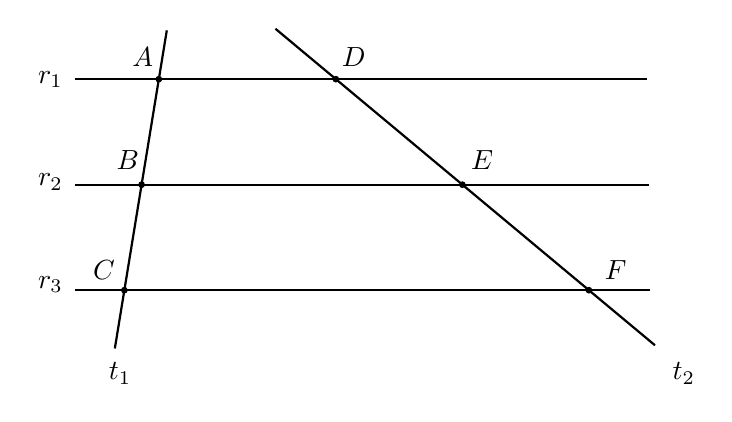
\begin{tikzpicture}
\draw [line width=0.8pt] (-2.7,0.)-- (4.6,0.);
\draw [line width=0.8pt] (-2.7,2.68)-- (4.56,2.68);
\draw [line width=0.8pt] (-2.7,1.34)-- (4.58,1.34);
\draw [line width=0.8pt] (-1.54,3.3)-- (-2.2,-0.74);
\draw [line width=0.8pt] (-0.16,3.32)-- (4.66,-0.7);
\draw (-2.1,3.2) node[anchor=north west] {$A$};
\draw (-2.3,1.9) node[anchor=north west] {$B$};
\draw (-2.6,0.5) node[anchor=north west] {$C$};
\draw (0.558,3.2) node[anchor=north west] {$D$};
\draw (2.2,1.9) node[anchor=north west] {$E$};
\draw (3.9,0.5) node[anchor=north west] {$F$};
\draw (-3.3,2.9) node[anchor=north west] {$r_1$};
\draw (-3.3,1.6) node[anchor=north west] {$r_2$};
\draw (-3.3,0.3) node[anchor=north west] {$r_3$};
\draw (-2.4,-0.8) node[anchor=north west] {$t_1$};
\draw (4.76,-0.8) node[anchor=north west] {$t_2$};
\draw [fill=black] (-1.6412871287128707,2.68) circle (1.0pt);
\draw [fill=black] (-1.86019801980198,1.34) circle (1.0pt);
\draw [fill=black] (-2.079108910891089,0.) circle (1.0pt);
\draw [fill=black] (0.6073631840796017,2.68) circle (1.0pt);
\draw [fill=black] (2.214029850746268,1.34) circle (1.0pt);
\draw [fill=black] (3.8206965174129355,0.) circle (1.0pt);
\end{tikzpicture}\end{center}
O enunciado pede que você demonstre uma afirmação. Em Matemática, demonstrar significa justificar a afirmação utilizando argumentos lógicos baseados em fatos conhecidos anteriormente.

Faremos, a seguir, perguntas que são dicas para ajudá-lo a demonstrar essa proposição.

Vamos considerar, na figura dada, \(AB=BC\). Não haveria diferença, caso escolhêssemos considerar \(DE=EF\) na outra trasnversal. Com os elementos da figura acima, responda:
\begin{enumerate}
\item {} 
O que se deseja demonstrar?

Para conseguir os argumentos necessários você vai ter que interferir na figura. Faça o seguinte:
\begin{itemize}
\item {} 
Trace por \(D\) uma paralela a \(t_1\) que intersecta \(r_2\) no ponto \(G\).

\item {} 
Trace por \(E\) uma paralela a \(t_1\) que intersecta \(r_3\) no ponto \(H\).

\end{itemize}

\item {} 
Os triângulos \(DGE\) e \(EHF\) são congruentes? Por quê?

\item {} 
O que se conclui da congruência dos triângulos \(DGE\) e \(EHF\)?

\end{enumerate}
\end{task}




\practice{}

\begin{task}{dividindo um segmento em partes iguais}

Um segmento desenhado no papel precisa ser dividido em três partes iguais. Um aluno fez assim:

Com uma régua mediu seu comprimento encontrando \(7{,}1\) cm.

Com a calculadora dividiu essa medida por $3$.

Ele pretende usar a régua para aplicar sobre o segmento a medida que aparece na calculadora.
\begin{enumerate}
\item {} 
Que número o visor da calculadora mostrou quando o segmento dado foi dividido por $3$?

\item {} 
Você consegue, com a régua escolar, marcar sobre o segmento a medida que a calculadora mostrou?

\end{enumerate}

Você percebe aí uma dificuldade, não é mesmo? Nossos sentidos são limitados e a régua não marca com precisão medidas menores que $1$ milímetro. Como fazer então?

Buscamos  inspiração na atividade anterior. Considere a seguinte construção:

Nosso segmento chama-se \(AB\).
\begin{itemize}
\item {} 
A partir de \(A\) trace uma semirreta \(AX\) (que não contenha o segmento \(AB\)).

\item {} 
Com o compasso em uma abertura qualquer fixada, assinale, a partir de \(A\), três segmentos iguais. Chamaremos esses pontos sobre a semirreta \(AX\) de \(M\), \(N\) e \(P\). Veja a figura.

\end{itemize}
\begin{center}\begin{tikzpicture}
\draw [line width=0.8pt] (0.,0.)-- (4.5,0.);
\draw [line width=0.8pt] (0.,0.)-- (6.38,-3.18);
\draw (1.46,-1.04) node[anchor=north west] {$M$};
\draw (3.26,-1.88) node[anchor=north west] {$N$};
\draw (5.08,-2.8) node[anchor=north west] {$P$};
\draw (6.5,-2.96) node[anchor=north west] {$X$};
\draw [line width=0.8pt] (0.,0.)-- (1.7450813116921962,-0.8698054186804365);
\draw [line width=0.8pt] (0.8813642797528934,-0.33874063957697237) -- (0.8010678993991632,-0.4998384089659029);
\draw [line width=0.8pt] (0.9440134122930329,-0.369967009714534) -- (0.8637170319393028,-0.5310647791034646);
\draw [line width=0.8pt] (1.7450813116921962,-0.8698054186804365)-- (3.4901626233843923,-1.739610837360873);
\draw [line width=0.8pt] (2.6264455914450897,-1.2085460582574088) -- (2.546149211091359,-1.3696438276463392);
\draw [line width=0.8pt] (2.6890947239852294,-1.2397724283949703) -- (2.608798343631499,-1.4008701977839009);
\draw [line width=0.8pt] (3.4901626233843923,-1.739610837360873)-- (5.235243935076588,-2.6094162560413094);
\draw [line width=0.8pt] (4.371526903137285,-2.078351476937845) -- (4.291230522783555,-2.239449246326776);
\draw [line width=0.8pt] (4.4341760356774245,-2.1095778470754065) -- (4.353879655323694,-2.2706756164643376);
\draw [fill=black] (0.,0.) circle (1.0pt);
\draw[color=black] (-0.06,0.31) node {$A$};
\draw [fill=black] (4.5,0.) circle (1.0pt);
\draw[color=black] (4.46,0.33) node {$B$};
\draw [fill=black] (1.7450813116921962,-0.8698054186804365) circle (2.0pt);
\draw [fill=black] (3.4901626233843923,-1.739610837360873) circle (2.0pt);
\draw [fill=black] (5.235243935076588,-2.6094162560413094) circle (2.0pt);
\end{tikzpicture}\end{center}
Em seguida, trace a reta \(PB\) e trace paralelas a ela pelos pontos \(M\) e \(N\). Essas paralelas intersectarão o segmento \(AB\) nos pontos \(C\) e \(D\), como mostra a figura.
\begin{center}\begin{tikzpicture}
\draw [line width=0.8pt] (0.,0.)-- (4.5,0.);
\draw [line width=0.8pt] (0.,0.)-- (6.38,-3.18);
\draw (1.46,-1.04) node[anchor=north west] {$M$};
\draw (3.26,-1.88) node[anchor=north west] {$N$};
\draw (5.08,-2.8) node[anchor=north west] {$P$};
\draw (6.5,-2.96) node[anchor=north west] {$X$};
\draw [line width=0.8pt] (0.,0.)-- (1.7450813116921962,-0.8698054186804365);
\draw [line width=0.8pt] (0.8813642797528934,-0.33874063957697215) -- (0.8010678993991632,-0.49983840896590276);
\draw [line width=0.8pt] (0.9440134122930329,-0.3699670097145338) -- (0.8637170319393028,-0.5310647791034644);
\draw [line width=0.8pt] (1.7450813116921962,-0.8698054186804365)-- (3.4901626233843923,-1.739610837360873);
\draw [line width=0.8pt] (2.6264455914450897,-1.2085460582574086) -- (2.546149211091359,- 1.3696438276463392);
\draw [line width=0.8pt] (2.6890947239852294,-1.2397724283949703) -- (2.608798343631499,-1.4008701977839009);
\draw [line width=0.8pt] (3.4901626233843923,-1.739610837360873)-- (5.235243935076588,-2.6094162560413094);
\draw [line width=0.8pt] (4.371526903137285,-2.078351476937845) -- (4.291230522783555,-2.239449246326776);
\draw [line width=0.8pt] (4.4341760356774245,-2.1095778470754065) -- (4.353879655323694,-2.2706756164643376);
\draw [line width=0.8pt,dash pattern=on 1pt off 1pt,color=session1] (4.5,0.)--  (5.235243935076588,-2.6094162560413094);
\draw [line width=0.8pt,dash pattern=on 1pt off 1pt,color=session1] (1.7450813116921962,-0.8698054186804365)-- (1.5,0.);
\draw [line width=0.8pt,dash pattern=on 1pt off 1pt,color=session1] (3.4901626233843923,-1.739610837360873)-- (3.,0.);
\draw [color=session3](1.34,0.6) node[anchor=north west] {C};
\draw [color=session3](2.88,0.6) node[anchor=north west] {D};
\draw [fill=black] (0.,0.) circle (1.0pt);
\draw[color=black] (-0.06,0.31) node {$A$};
\draw [fill=black] (4.5,0.) circle (1.0pt);
\draw[color=black] (4.46,0.33) node {$B$};
\draw [fill=black] (1.7450813116921962,-0.8698054186804365) circle (1.0pt);
\draw [fill=black] (3.4901626233843923,-1.739610837360873) circle (1.0pt);
\draw [fill=black] (5.235243935076588,-2.6094162560413094) circle (1.0pt);
\draw [fill=session3] (1.5,0.) circle (1.5pt);
\draw [fill=session3] (3.,0.) circle (1.5pt);
\end{tikzpicture}
\end{center}

\begin{enumerate}\setcounter{enumi}{2}
\item {} 
Com esse procedimento, explique por que os pontos \(C\) e \(D\) dividem o segmento \(AB\) em três partes iguais.

\item {} 
Para dividir um segmento em partes iguais há necessidade de fazer medidas?

\end{enumerate}
\end{task}


\clearpage
\arrange{o que é um teorema?}

\clearmargin
\begin{objectives}{Segmentos comensuráveis}
{
Levar o estudante a
\begin{itemize}
\item {} 
Identificar uma unidade comum a dois segmentos cujas medidas são racionais.

\end{itemize}
}{1}{2}
\end{objectives}
\begin{sugestions}{Segmentos comensuráveis}
{
\begin{itemize}
\item {} 
Quando as medidas dos dois segmentos são números racionais apresentados com representações decimais, os alunos não terão o menor problema em obter uma unidade comum para esses segmentos.

\item {} 
Quando as medidas são números racionais dados por meio da representação fracionária, a dica é obter frações equivalentes com o mesmo denominador. A unidade comum fica óbvia.

\item {} 
É necessário comentar que dois segmentos nem sempre admitem uma unidade comum. Por exemplo, se um segmento mede 1 unidade e outro mede \(\sqrt{2}\) unidades, não existe uma unidade comum. Neste capítulo vamos abordar, inicialmente, a demonstração do teorema de Tales no caso dos segmentos comensuráveis. A demonstração geral aparecerá no final do capítulo..

\end{itemize}
}{1}{2}
\end{sugestions}
\begin{answer}{Segmentos comensuráveis}
{
As respostas são pessoais. Daremos a menor unidade para cada um dos casos.
\begin{enumerate}
\item {} 
0,1

\item {} 
0,01

\item {} 
0,001

\item {} 
0,0001

\item {} 
1/30

\end{enumerate}
}{1}
\end{answer}
\begin{objectives}{Compreendendo o teorema de Tales}
{
\begin{itemize}
\item {} 
Compreender o enunciado do teorema de Tales identificando   a hipótese e a tese

\end{itemize}
}{1}{2}
\end{objectives}
\begin{sugestions}{Compreendendo o teorema de Tales}
{
\begin{itemize}
\item {} 
É necessário rever o que é uma proporcionalidade e o que significa dizer que  segmentos dados sejam proporcionais a outros também dados.

\item {} 
Exemplos devem ser dados. Se o professor disser que, sobre uma das transversais, um segmento é o dobro do outro, os alunos deverão concluir que, na outra trasnversal, os segmentos correspondentes serão um o dobro do outro.

\end{itemize}
}{1}{1}
\end{sugestions}
\begin{answer}{Compreendendo o teorema de Tales}
{
\begin{enumerate}
\item {} 
As retas paralelas são cortadas por transversais.

\item {} 
\(\dfrac{a}{a'}=\dfrac{b}{b'}=\dfrac{c}{c'}\)

\end{enumerate}
}{1}
\end{answer}
\begin{objectives}{Demonstrando o teorema de Tales}
{
\begin{itemize}
\item {} 
Demonstrar o teorema de Tales no caso dos segmentos comensuráveis.

\end{itemize}
}{1}{1}
\end{objectives}
\begin{sugestions}{Demonstrando o teorema de Tales}
{
\begin{itemize}
\item {} 
O aluno fará a demonstração do teorema de Tales no caso em que os dois segmentos da primeira transversal são comensuráveis.

\end{itemize}

O texto dirá que o resultado vale quando as medidas dos segmentos são números reais quaisquer. Uma demonstração geral do teorema de Tales usando áreas estará no Para Saber Mais, no final do capítulo.
}{1}{1}
\end{sugestions}
\clearmargin
\begin{answer}{Demonstrando o teorema de Tales}
{
\begin{enumerate}
\item {} 
\(m\)

\item {} 
\(n\)

\item {} 
\(a'= mv\) e \(b'=nv\)

Tomando a razão entre os elementos do lado esquerdo e os do lado direito, obtemos \(\dfrac{a}{a'}=\dfrac{mu}{nu}=\dfrac{m}{n}\) e que \(\dfrac{b}{b'}=\dfrac{mv}{nv}=\dfrac{m}{n}\), logo \(\dfrac{a}{a'}=\dfrac{b}{b'}\)

\end{enumerate}
}{1}
\end{answer}




Na atividade anterior você fez uma demonstração. Havia três retas paralelas intersectadas por duas transversais e você considerou, naquela situação que  \(AB = BC\). Assim, o fato a ser demonstrado era que \(DE = EF\).

Um \textbf{TEOREMA} é uma afirmação matemática que precisa de uma justificativa para ser aceita.

Em um teorema, a situação e os fatos que são dados constituem a \textbf{HIPÓTESE}. O fato que que se quer demonstrar é a \textbf{TESE}.

A partir da hipótese e para concluir a tese há um caminho composto por argumentos sucessivos, onde cada um é consequência dos anteriores. Esse caminho é a \textbf{DEMONSTRAÇÃO}.

Uma forma comum de enunciar um teorema é:

Se  \textbf{Hipótese},  então \textbf{Tese}.

\begin{example}{Teorema de Pitágoras}
Como exemplo, o famoso teorema de Pitágoras diz que:

“Se \textbf{um triângulo é retângulo} então \textbf{o quadrado da hipotenusa é igual à soma dos quadrados dos catetos}”.

Podemos separar:

\textbf{Hipótese}: um triângulo é retângulo

\textbf{Tese}: o quadrado da hipotenusa é igual à soma dos quadrados dos catetos
\end{example}

O objetivo deste capítulo é compreender o “teorema de Tales”. Esse é um teorema muito antigo e importante, pois com ele, diversas outras propriedades de figuras da geometria foram demonstradas. O enunciado do teorema que vamos apresentar a seguir inclui a palavra “feixe”. Entenda essa palavra como “conjunto”.

Razão entre segmentos

É preciso explicar certos termos que usamos em geometria. Eles são muito antigos, mas são usados hoje e serão sempre.

A razão entre dois segmentos é a razão entre suas medidas.

Por exemplo, se um segmento \(x\) mede $15$ cm e um segmento \(y\) mede $20$ cm, a razão entre eles é escrita como \(\frac{x}{y}\) e é igual a \(\frac{15}{20}=\frac{3}{4}=0,75\).

Quando um ponto \(P\) está no interior do segmento \(AB\), para definir sua posição em relação aos extremos do segmento é costume definir um número chamado de “razão em que \(P\) divide o segmento \(AB\)”.

Essa razão é o número real \(\frac{PA}{PB}\).

Assim, se um segmento \(AB\) mede \(10\)cm e um ponto \(P\) sobre ele está a $4$ cm de A então a razão em que \(P\) divide esse segmento é \(\frac{PA}{PB}=\frac{4}{6}=\frac{2}{3}\).
\begin{center}\begin{tikzpicture}
\draw [line width=0.8pt] (0,0)-- (10,0);
\draw (1.7,.7) node[anchor=north west] {4};
\draw (7.2,.7) node[anchor=north west] {6};
\draw [fill=black] (0,0) circle (1.0pt);
\draw[color=black] (0,-0.5) node {$A$};
\draw [fill=black] (10,0.) circle (1.0pt);
\draw[color=black] (10,-0.5) node {$B$};
\draw [fill=black] (4,0.) circle (1.0pt);
\draw[color=black] (4,-0.5) node {$P$};
\end{tikzpicture}\end{center}
Isso pode ser visualizado na figura a seguir onde o segmento \(PA\) contém 2 partes e o segmento \(PB\), 3 partes.
\begin{center}\begin{tikzpicture}
\definecolor{ffqqqq}{rgb}{1.,0.,0.}
\draw [line width=0.8pt] (0.,0.)-- (10.,0.);
\draw [line width=.5pt,dashed,color=ffqqqq] (0.,0.4)-- (2.,0.4);
\draw [line width=.5pt,dashed,color=ffqqqq] (2.,0.4)-- (4.,0.4);
\draw [line width=.5pt,dashed,color=ffqqqq] (4.,0.4)-- (6.,0.4);
\draw [line width=.5pt,dashed,color=ffqqqq] (6.,0.4)-- (8.,0.4);
\draw [line width=.5pt,dashed,color=ffqqqq] (8.,0.4)-- (10.,0.4);
\draw (0.7,0.8) node[anchor=north west] {$a$};
\draw (2.7,0.8) node[anchor=north west] {$a$};
\draw (4.7,0.8) node[anchor=north west] {$a$};
\draw (6.7,0.8) node[anchor=north west] {$a$};
\draw (8.7,0.8) node[anchor=north west] {$a$};
\draw [fill=black] (0.,0.) circle (1.0pt);
\draw[color=black] (-0.1322345939243572,-0.7290716059761639) node {$A$};
\draw [fill=black] (10.,0.) circle (1.0pt);
\draw[color=black] (9.974376348759716,-0.7290716059761639) node {$B$};
\draw [fill=black] (4.,0.) circle (1.0pt);
\draw[color=black] (4.004668330801247,-0.6767057461695107) node {$P$};
\draw [color=black] (0.,0.4)-- ++(-2.5pt,0 pt) -- ++(5.0pt,0 pt) ++(-2.5pt,-2.5pt) -- ++(0 pt,5.0pt);
\draw [color=black] (2.,0.4)-- ++(-2.5pt,0 pt) -- ++(5.0pt,0 pt) ++(-2.5pt,-2.5pt) -- ++(0 pt,5.0pt);
\draw [color=black] (4.,0.4)-- ++(-2.5pt,0 pt) -- ++(5.0pt,0 pt) ++(-2.5pt,-2.5pt) -- ++(0 pt,5.0pt);
\draw [color=black] (6.,0.4)-- ++(-2.5pt,0 pt) -- ++(5.0pt,0 pt) ++(-2.5pt,-2.5pt) -- ++(0 pt,5.0pt);
\draw [color=black] (8.,0.4)-- ++(-2.5pt,0 pt) -- ++(5.0pt,0 pt) ++(-2.5pt,-2.5pt) -- ++(0 pt,5.0pt);
\draw [color=black] (10.,0.4)-- ++(-2.5pt,0 pt) -- ++(5.0pt,0 pt) ++(-2.5pt,-2.5pt) -- ++(0 pt,5.0pt);
\end{tikzpicture}\end{center}
\begin{task}{segmentos comensuráveis}



Dois segmentos são chamados de comensuráveis quando é possível determinar um terceiro segmento que cabe exatamente um número inteiro de vezes em um deles e também um número inteiro de vezes no outro.

Assim, dados dois segmentos \(a\) e \(b\), um segmento que cabe um número inteiro de vezes em um deles e também um número inteiro de vezes no outro é chamado de uma \textit{unidade}, e vamos representá-lo por \(u\).

Por exemplo, se \(a = 8\) cm e \(b = 10\) cm a unidade \(u = 1\) cm cabe 8 vezes em \(a\) e 10 vezes em \(b\), mas podemos tomar \(u = 2\) cm pois essa unidade cabe 4 vezes em \(a\) e 5 vezes em \(b\). . Porém, há outras opções para \(u\), que dependem da escolha de cada pessoa. Com esses mesmos segmentos, podemos escolher, por exemplo,  \(u = 0{,}5\) cm e assim, essa unidade cabe 16 vezes em \(a\) e 20 vezes em \(b\).
Esses são os segmentos comensuráveis: os segmentos que permitem encontrar uma unidade de medida comum.

Responda

Na tabela abaixo, para cada par de segmentos \(a\) e \(b\), com suas medidas dadas em centímetros,  encontre uma unidade \(u\) de medida comum de forma que ela caiba um número inteiro de vezes em cada um deles..
\end{task}




\begin{task}{compreendendo o teorema de Tales}



Enunciado do teorema de Tales:

“Se um feixe de paralelas está cortado por duas transversais então os segmentos determinados sobre uma transversal são respectivamente proporcionais aos segmentos determinados na outra”.

Vejamos uma figura
\begin{center}\begin{tikzpicture}
\draw [line width=0.8pt] (-3.24,0.)-- (4.8,0.);
\draw [line width=0.8pt] (-3.3,4.22)-- (4.82,4.22);
\draw [line width=0.8pt] (-3.28,3.02)-- (4.8,3.02);
\draw [line width=0.8pt] (-3.26,2.32)-- (4.82,2.32);
\draw [line width=0.8pt] (-2.68,4.76)-- (-1.26,-0.56);
\draw [line width=0.8pt] (-1.42,4.84)-- (4.78,-0.64);
\draw [line width=2.pt,color=session1] (-2.535864661654135,4.22)-- (-2.215563909774436,3.02);
\draw [line width=2.pt,color=session3] (-2.215563909774436,3.02)-- (-2.0287218045112776,2.32);
\draw [line width=2.pt,color=session2] (-2.0287218045112776,2.32)-- (-1.4094736842105262,0.);
\draw [line width=2.pt,color=session1] (-0.7185401459854013,4.22)-- (0.6391240875912405,3.02);
\draw [line width=2.pt,color=session3] (0.6391240875912405,3.02)-- (1.4310948905109493,2.32);
\draw [line width=2.pt,color=session2] (1.4310948905109493,2.32)-- (4.0559124087591245,0.);
\draw (-2.9,3.9) node[anchor=north west] {$ a $};
\draw (0.1,4) node[anchor=north west] {$ a' $};
\draw (-2.6,3) node[anchor=north west] {$ b $};
\draw (1.2,3.0) node[anchor=north west] {$ b' $};
\draw (-2.2,1.4) node[anchor=north west] {$c$};
\draw (2.9,1.7) node[anchor=north west] {$ c' $};
\draw [fill=black] (-2.535864661654135,4.22) circle (1.0pt);
\draw [fill=black] (-2.215563909774436,3.02) circle (1.0pt);
\draw [fill=black] (-2.0287218045112776,2.32) circle (1.0pt);
\draw [fill=black] (-1.4094736842105262,0.) circle (1.0pt);
\draw [fill=black] (-0.7185401459854013,4.22) circle (1.0pt);
\draw [fill=black] (0.6391240875912405,3.02) circle (1.0pt);
\draw [fill=black] (1.4310948905109493,2.32) circle (1.0pt);
\draw [fill=black] (4.0559124087591245,0.) circle (1.0pt);
\end{tikzpicture}\end{center}
Responda considerando a figura acima
\begin{enumerate}
\item {} 
Qual é a hipótese do teorema?

\item {} 
Qual é a tese do teorema?

\end{enumerate}
\end{task}


\begin{task}{demonstrando o teorema de Tales}

A figura a seguir mostra três retas paralelas cortadas por duas transversais. Na reta da esquerda, os segmentos \(AB = a\) e \(BC = b\), são comensuráveis e, na reta da direita, os segmentos correspondentes são \(A'B' = a'\) e \(B'C' = b'\).
Nosso objetivo é demonstrar que
\begin{equation*}
\begin{split}\frac{a}{a'}=\frac{b}{b'}\end{split}
\end{equation*}
Como \(a\) e \(b\) são comensuráveis, a figura mostra uma unidade \(u\) comum a esses segmentos.

Por cada extremidade da unidade \(u\) assinalada na reta da esquerda traçamos retas paralelas às retas dadas determinando segmentos correspondentes na reta da direita.

Digamos que a unidade \(u\) cabe \(m\) vezes em \(a\). Então \(a = mu\).

Digamos que a unidade \(u\) cabe \(n\) vezes em \(b\). Então \(b = nu\).

Sabemos (da atividade \hyperref[demonstrando-afirmacao]{"Demonstrando um Fato"}) que, em retas paralelas cortadas por transversais, segmentos iguais de um lado correspondem a segmentos iguais do outro. A cada segmento \(u\) do lado esquerdo existe um correspondente \(v\) do lado direito.


\begin{center}\begin{tikzpicture}
\draw [line width=0.8pt] (-3.56,0.)-- (5.52,0.);
\draw [line width=0.8pt] (-3.44,3.8)-- (5.34,3.8);
\draw [line width=0.8pt] (-3.36,6.38)-- (5.3,6.38);
\draw [line width=0.8pt] (-1.98,6.94)-- (-3.06,-0.72);
\draw [line width=0.8pt] (-0.78,6.94)-- (5.36,-0.74);
\draw [line width=2.4pt,color=session3] (-2.058955613577024,6.38)-- (-2.120786270710496,5.941460339220002);
\draw [line width=2.4pt,color=session3] (-2.120786270710496,5.941460339220002)-- (-2.1826169278439687,5.502920678440002);
\draw [line width=0.8pt] (-2.1826169278439687,5.502920678440002)-- (-2.2444475849774412,5.064381017660003);
\draw [line width=2.4pt,color=session3] (-2.422715404699739,3.8)-- (-2.484546061833212,3.361460339220001);
\draw [line width=2.4pt,color=session2] (-0.33229166666666593,6.38)-- (0.018311655884010396,5.941460339220002);
\draw [line width=2.4pt,color=session2] (0.018311655884010396,5.941460339220002)-- (0.3689149784346872,5.502920678440002);
\draw [line width=2.4pt,color=session2] (1.7303645833333339,3.8)-- (2.0809679058840103,3.361460339220001);
\draw [line width=0.8pt,dash pattern=on 1pt off 1pt,color=session1] (-2.120786270710496,5.941460339220002)-- (0.018311655884010396,5.941460339220002);
\draw [line width=0.8pt,dash pattern=on 1pt off 1pt,color=session1] (-2.1826169278439687,5.502920678440002)-- (0.3689149784346872,5.502920678440002);
\draw [line width=0.8pt,dash pattern=on 1pt off 1pt,color=session1] (-2.2444475849774412,5.064381017660003)-- (0.7195183009853631,5.064381017660003);
\draw [line width=0.8pt,dash pattern=on 1pt off 1pt,color=session1] (-2.360884747566267,4.238539660779997)-- (1.3797612607826595,4.238539660779998);
\draw [line width=0.8pt,dash pattern=on 1pt off 1pt,color=session1] (-2.484546061833212,3.361460339220001)-- (2.0809679058840103,3.361460339220001);
\draw [line width=0.8pt,dash pattern=on 1pt off 1pt,color=session1] (-2.5463767189666844,2.9229206784400033)-- (2.431571228434686,2.922920678440003);
\draw [line width=0.8pt,dash pattern=on 1pt off 1pt,color=session1] (-2.608207376100157,2.4843810176600054)-- (2.7821745509853613,2.4843810176600054);
\draw [line width=0.8pt,dash pattern=on 1pt off 1pt,color=session1] (-2.83482432541974,0.8770793215599975)-- (4.067178771565316,0.8770793215599976);
\draw [line width=0.8pt,dash pattern=on 1pt off 1pt,color=session1] (-2.896654982553212,0.43853966077999873)-- (4.417782094115991,0.43853966077999873);
\draw (-2.5,6.9) node[anchor=north west] {$A$};
\draw (-2.9,4.3) node[anchor=north west] {$B$};
\draw (-3.6,0.6) node[anchor=north west] {$C$};
\draw (-0.2,6.9) node[anchor=north west] {$A'$};
\draw (1.8,4.3) node[anchor=north west] {$B'$};
\draw (4.8,0.6) node[anchor=north west] {$C'$};
\draw (-2.6,6.4) node[anchor=north west] {$  u$};
\draw (-3,3.8) node[anchor=north west] {$ u$};
\draw (-.1,6.4) node[anchor=north west] {$ v $};
\draw (1.9,3.8) node[anchor=north west] {$ v $};
\draw (-3.1111119322537544,5.579654794304461) node[anchor=north west] {$ a $};
\draw (-3.5150523810387724,2.4603368842423774) node[anchor=north west] {$ b $};
\draw (1.4668798206431133,5.736742746609745) node[anchor=north west] {$ a' $};
\draw (3.7558756970915472,2.617424836547662) node[anchor=north west] {$  b'$};
\draw [fill=black] (-2.058955613577024,6.38) circle (2.0pt);
\draw [fill=black] (-0.33229166666666593,6.38) circle (2.0pt);
\draw [fill=black] (-2.422715404699739,3.8) circle (2.0pt);
\draw [fill=black] (1.7303645833333339,3.8) circle (2.0pt);
\draw [fill=black] (-2.958485639686684,0.) circle (2.0pt);
\draw [fill=black] (4.768385416666668,0.) circle (2.0pt);
\draw [fill=black] (-2.120786270710496,5.941460339220002) circle (2.0pt);
\draw [fill=black] (-2.1826169278439687,5.502920678440002) circle (2.0pt);
\draw [fill=black] (-2.2444475849774412,5.064381017660003) circle (2.0pt);
\draw [fill=black] (-2.360884747566267,4.238539660779997) circle (2.0pt);
\draw [fill=black] (-2.484546061833212,3.361460339220001) circle (2.0pt);
\draw [fill=black] (-2.896654982553212,0.43853966077999873) circle (2.0pt);
\draw [fill=black] (-2.5463767189666844,2.9229206784400033) circle (2.0pt);
\draw [fill=black] (-2.608207376100157,2.4843810176600054) circle (2.0pt);
\draw [fill=black] (-2.83482432541974,0.8770793215599975) circle (2.0pt);
\draw [fill=black] (0.018311655884010396,5.941460339220002) circle (2.0pt);
\draw [fill=black] (0.3689149784346872,5.502920678440002) circle (2.0pt);
\draw [fill=black] (0.7195183009853631,5.064381017660003) circle (2.0pt);
\draw [fill=black] (1.3797612607826595,4.238539660779998) circle (2.0pt);
\draw [fill=black] (2.0809679058840103,3.361460339220001) circle (2.0pt);
\draw [fill=black] (2.431571228434686,2.922920678440003) circle (2.0pt);
\draw [fill=black] (2.7821745509853613,2.4843810176600054) circle (2.0pt);
\draw [fill=black] (4.067178771565316,0.8770793215599976) circle (2.0pt);
\draw [fill=black] (4.417782094115991,0.43853966077999873) circle (2.0pt);
\end{tikzpicture}\end{center}

Complete a demonstração


\begin{enumerate}
\item {} 
Quantas vezes o segmento \(v\) cabe em \(a'\)?

\item {} 
Quantas vezes o segmento \(v\) cabe em \(b'\)?

\item {} 
Escreva as medidas de \(a'\) e \(b'\) na unidade \(v\), reuna essas medidas com as anteriores e conclua o resultado do teorema

\end{enumerate}
\end{task}



\begin{observation}{}

O teorema de Tales foi demonstrado no caso dos dois segmentos de uma das retas serem comensuráveis. Entretanto, o teorema vale quando as medidas desses dois segmentos são números reais quaisquer. A demonstração geral do teorema está no final do capítulo, na seção Para Saber Mais.
\end{observation}

\clearpage
\def\currentcolor{session2}
\begin{objectives}{Resolvendo a situação inicial}
{
\begin{itemize}
\item {} 
Reconhecer a aplicabilidade do teorema de Tales em uma situação real.

\end{itemize}
}{1}{1}
\end{objectives}
\begin{sugestions}{Resolvendo a situação inicial}
{
\begin{itemize}
\item {} 
Os alunos devem perceber que os segmentos que aparecem nas transversais não precisam estar conectados.

\item {} 
Deixe que os alunos concluam o resultado e encontrem a resposta. Não dê nenhuma dica inicialmente.

\end{itemize}
}{1}{1}
\end{sugestions}
\begin{answer}{Resolvendo a situação inicial}
{
\begin{enumerate}
\item {} 
Porque as ruas são paralelas e estão cortadas por transversais.

\item {} 
\(184m\)

\end{enumerate}
}{1}
\end{answer}
\begin{objectives}{Resolvendo novas situações}
{
\begin{itemize}
\item {} 
Reconhecer uma aplicação do teorema de Tales em uma situação matemática.

\end{itemize}
}{1}{1}
\end{objectives}
\begin{sugestions}{Resolvendo novas situações}
{
\begin{itemize}
\item {} 
Os alunos compreenderam o teorema de Tales a partir da representação mais tradicional. Nesta atividade, vamos variar as situações propostas para que eles possam raciocinar e decidir como aplicar o teorema de Tales

\item {} 
Em caso de dificuldade sugira que eles tracem uma nova paralela pelo ponto de interseção dos segmentos. Eles deverão reconhecer, então, o teorema de Tales.

\end{itemize}
}{1}{1}
\end{sugestions}
\clearmargin
\begin{answer}{Resolvendo novas situações}
{
\begin{enumerate}
\item {} 
5,25

\item {} 
\(\dfrac{a}{d}=\dfrac{c}{b}\)

\end{enumerate}
}{1}
\end{answer}


\practice{}

\begin{task}{resolvendo a situação inicial}



Vamos voltar ao mapa que mostramos na primeira atividade, agora desenhado de forma esquemática.
\begin{center}\begin{tikzpicture}
\draw [line width=0.8pt] (0.,5.)-- (7.2,1.44);
\draw [line width=0.8pt] (0.,5.)-- (0.,-2.86);
\draw [line width=2.8pt,color=session3] (7.2,1.44)-- (5.629240434037691,-1.60334665905197);
\draw [line width=0.8pt] (5.629240434037691,-1.60334665905197)-- (4.7328383780696734,-3.3401256424900057);
\draw [line width=2.8pt,color=session1] (4.7328383780696734,-3.3401256424900057)-- (3.968018275271273,-4.821964591661907);
\draw [line width=0.8pt] (0.,3.22)-- (6.468075385494003,0.02189605939463218);
\draw [line width=0.8pt] (0.,1.18)-- (5.629240434037691,-1.60334665905197);
\draw [line width=0.8pt] (0.,2.86)-- (6.320045688178182,-0.2649114791547684);
\draw [line width=0.8pt] (0.,-1.)-- (4.7328383780696734,-3.3401256424900057);
\draw [line width=0.8pt] (0.,-2.86)-- (3.968018275271273,-4.821964591661907);
\draw [line width=2.8pt,color=session3] (0.,5.)-- (0.,1.18);
\draw [line width=2.8pt,color=session1] (0.,-1.)-- (0.,-2.86);
\draw [color=session1](4.4,-4.0) node[anchor=north west] {$A$};
\draw [color=session1](-0.6170786902907064,-1.7707838711724064) node[anchor=north west] {$B$};
\draw [color=session3](6.5,-0.3084989813871627) node[anchor=north west] {$C$};
\draw [color=session3](-0.6767637878329612,3.3322919686903827) node[anchor=north west] {$D$};
\draw [fill=session3] (0.,5.) circle (2.5pt);
\draw [fill=session3] (0.,1.18) circle (2.5pt);
\draw [fill=session1] (0.,-1.) circle (2.5pt);
\draw [fill=session1] (0.,-2.86) circle (2.5pt);
\draw [fill=session3] (7.2,1.44) circle (2.5pt);
\draw [fill=session3] (5.629240434037691,-1.60334665905197) circle (2.5pt);
\draw [fill=session1] (4.7328383780696734,-3.3401256424900057) circle (2.5pt);
\draw [fill=session1] (3.968018275271273,-4.821964591661907) circle (2.5pt);
\end{tikzpicture}\end{center}\begin{enumerate}
\item {} 
Por que o teorema de Tales pode ser utilizado nessa situação?

\item {} 
Utilizando os dados da atividade inicial (\hyperref[nas-ruas]{"Nas ruas de uma cidade"}) calcule a medida \(D\).

\end{enumerate}
\end{task}




\begin{task}{resolvendo novas situações}



Sempre que houver retas paralelas e trasnversais, o teorema de Tales estará presente. Nas figuras a seguir, as retas paralelas estão assinaladas com seu símbolo tradicional.
\begin{center}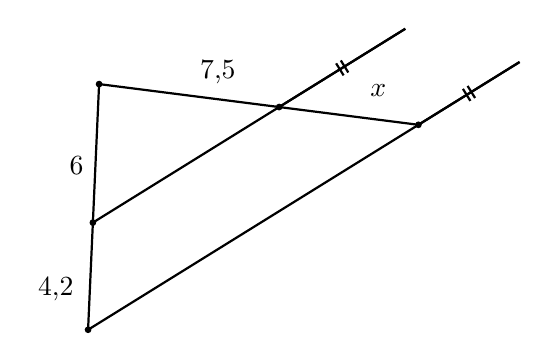
\begin{tikzpicture}
\draw [line width=0.8pt] (-2.04,0.56)-- (3.44,3.96);
\draw [line width=0.8pt] (-2.04,0.56)-- (-1.9,3.68);
\draw [line width=0.8pt] (-1.9,3.68)-- (2.1553812418250367,3.1629737631761174);
\draw [line width=0.8pt] (-1.9789362312897274,1.9208497026860774)-- (1.9886091282959177,4.382465436735565);
\draw [line width=0.8pt] (0.3865465119480187,3.3884849813372337)-- (1.9886091282959177,4.382465436735565);
\draw [line width=0.8pt] (1.1103882995267922,3.9434991515970954) -- (1.2052858218334364,3.7905466744675635);
\draw [line width=0.8pt] (1.1698698184104994,3.980403743605235) -- (1.2647673407171436,3.8274512664757028);
\draw [line width=0.8pt] (2.1553812418250367,3.1629737631761174)-- (3.44,3.96);
\draw [line width=0.8pt] (2.7205011003173425,3.6195108241487546) -- (2.8153986226239867,3.4665583470192227);
\draw [line width=0.8pt] (2.7799826192010486,3.6564154161568942) -- (2.8748801415076928,3.5034629390273624);
\draw (-2.4,2.88) node[anchor=north west] {6};
\draw (-2.8,1.34) node[anchor=north west] {4,2};
\draw (-0.74,4.1) node[anchor=north west] {7,5};
\draw (1.42,3.8) node[anchor=north west] {$ x $};
\draw [fill=black] (-2.04,0.56) circle (1.0pt);
\draw [fill=black] (-1.9,3.68) circle (1.0pt);
\draw [fill=black] (2.1553812418250367,3.1629737631761174) circle (1.0pt);
\draw [fill=black] (-1.9789362312897274,1.9208497026860774) circle (1.0pt);
\draw [fill=black] (0.3865465119480187,3.3884849813372337) circle (1.0pt);
\end{tikzpicture}\end{center}\begin{enumerate}
\item {} 
Qual é o valor da medida que está faltando na figura acima?

\end{enumerate}
\begin{center}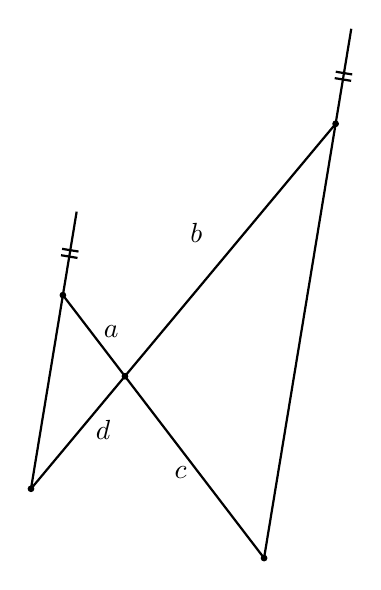
\begin{tikzpicture}
\draw [line width=0.8pt] (-2.8,1.)-- (1.0687644969670296,5.635260395386114);
\draw [line width=0.8pt] (-2.394800264009806,3.4591432253197976)-- (0.16,0.12);
\draw [line width=0.8pt] (-2.394800264009806,3.4591432253197976)-- (-2.22,4.52);
\draw [line width=0.8pt] (-2.418451428579632,3.9661819892341916) -- (-2.2097237468538884,3.9317893598589273);
\draw [line width=0.8pt] (-2.405076517155918,4.04735386546087) -- (-2.1963488354301743,4.012961236085605);
\draw [line width=0.8pt] (1.0687644969670296,5.635260395386114)-- (1.2676091397680478,6.8420416758336735);
\draw [line width=0.8pt] (1.0571355217928105,6.215261412184186) -- (1.265863203518554,6.180868782808922);
\draw [line width=0.8pt] (1.070510433216524,6.2964332884108645) -- (1.2792381149422676,6.2620406590356);
\draw [line width=0.8pt] (-2.8,1.)-- (-2.394800264009806,3.4591432253197976);
\draw [line width=0.8pt] (0.16,0.12)-- (1.0687644969670296,5.635260395386114);
\draw (-2,3.2) node[anchor=north west] {$ a $};
\draw (-0.9,4.5) node[anchor=north west] {$ b $};
\draw (-1.1,1.4) node[anchor=north west] {$ c $};
\draw (-2.1,2.0) node[anchor=north west] {$ d $};
\draw [fill=black] (-2.8,1.) circle (1.0pt);
\draw [fill=black] (0.16,0.12) circle (1.0pt);
\draw [fill=black] (1.0687644969670296,5.635260395386114) circle (1.0pt);
\draw [fill=black] (-2.394800264009806,3.4591432253197976) circle (1.0pt);
\draw [fill=black] (-1.6069520360906888,2.4294196457913784) circle (1.0pt);
\end{tikzpicture}\end{center}\begin{enumerate}
\item {} 
Encontre uma relação entre os quatro segmentos assinalados na figura acima.

\end{enumerate}
\end{task}



\arrange{}

\paragraph{Como se divide um segmento em uma razão dada?}

Imagine que tenhamos um segmento \(AB\) e desejamos determinar, no seu interior o ponto \(P\) que o divide na razão \(\frac{PA}{PB}=\frac{3}{4}\). Isso significa encontrar um ponto \(P\) no interior do segmento \(AB\) de forma que o segmento \(PA\) seja proporcional a 3 e o segmento \(PB\), proporcional a 4. Um procedimento bastante usado é o descrito a seguir e mostrado na figura a seguir à esquerda.

A partir dos pontos \(A\) e \(B\) trace semirretas paralelas quaisquer,{}`AX{}` e \(BY\),  mas com sentidos opostos como ilustrado na figura.
Usando o compasso com uma abertura qualquer,mas fixada, assinale três segmentos iguais e consecutivos na semirreta de origem  \(A\) e, com a mesma abertura do compasso, quatro segmentos na semirreta de origem \(B\).

Temos então \(AX = 3u\) e \(BY = 3u\).

A interseção da reta \(XY\) com o segmento \(AB\) é o ponto \(P\) procurado.
\begin{center}\begin{tikzpicture}
\draw [line width=0.8pt] (-3.,0.)-- (-1.62,2.92);
\draw [line width=0.8pt] (-3.,0.)-- (1.,0.);
\draw [line width=0.8pt] (3.,0.)-- (7.,0.);
\draw [line width=0.8pt] (1.,0.)-- (-0.502351497488208,-3.178888675844614);
\draw [line width=0.8pt] (-2.1744449131418495,1.746826705525942)-- (-0.10074011581086806,-2.3291022740345904);
\draw [line width=0.8pt] (3.8255550868581505,1.7468267055259423)-- (5.899259884189131,-2.3291022740345904);
\draw [line width=0.8pt] (3.,0.)-- (4.228558269739617,2.59955807799977);
\draw [line width=0.8pt] (7.,0.)-- (4.767191011235955,-4.724494382022471);
\draw [line width=0.8pt,dash pattern=on 1pt off 1pt] (2.7729644593415306,0.4462451650548752)-- (5.372740816526203,-4.663693244820947);
\draw [line width=0.8pt,dash pattern=on 1pt off 1pt] (3.0256681798973055,1.072708419540557)-- (5.649835588579647,-4.085171333659179);
\draw [line width=0.8pt,dash pattern=on 1pt off 1pt] (3.2905674262019144,1.6752010023642823)-- (5.959404510836151,-3.570478338777889);
\draw [line width=0.8pt,dash pattern=on 1pt off 1pt] (3.5514960008445655,2.2854980594391745)-- (6.1918296069376995,-2.904156839673689);
\draw [line width=0.8pt,dash pattern=on 1pt off 1pt] (4.187082831957212,2.159393075614541)-- (6.562234402556889,-2.509038578647954);
\draw [line width=0.8pt,dash pattern=on 1pt off 1pt] (4.762684778290206,2.1511901820602617)-- (6.823021221818061,-1.8984628971188342);
\draw [line width=0.8pt,dash pattern=on 1pt off 1pt] (5.34265446345135,2.1344023668297014)-- (7.096003566828064,-1.3118578872516715);
\draw [line width=0.8pt,dash pattern=on 1pt off 1pt] (5.937130743373617,2.0891014044734284)-- (7.329336201567188,-0.6473201825610867);
\draw (-3.44364,0.06722) node[anchor=north west] {A};
\draw (2.5991,0.01398) node[anchor=north west] {A};
\draw (1.21486,0.20032) node[anchor=north west] {B};
\draw (7.2576,0.06722) node[anchor=north west] {B};
\draw (-2.48532,2.32992) node[anchor=north west] {X};
\draw (3.29122,2.06442) node[anchor=north west] {X};
\draw (0.04358,-2.59478) node[anchor=north west] {Y};
\draw (6.00646,-2.38182) node[anchor=north west] {Y};
\draw (-3.2573,0.62624) node[anchor=north west] {u};
\draw (0.97528,-0.33208) node[anchor=north west] {u};
\draw [color=session3](-1.527,-0.2256) node[anchor=north west] {P};
\draw [color=session3](4.51574,-0.2256) node[anchor=north west] {P};
\draw [fill=black] (-3.,0.) circle (1.0pt);
\draw [fill=black] (1.,0.) circle (1.0pt);
\draw [fill=black] (3.,0.) circle (1.0pt);
\draw [fill=black] (7.,0.) circle (1.0pt);
\draw [fill=black] (-2.724814971047283,0.5822755685086475) circle (1.0pt);
\draw [fill=black] (-2.449629942094566,1.1645511370172947) circle (1.0pt);
\draw [fill=black] (-3.,0.) circle (1.0pt);
\draw [fill=black] (-2.1744449131418495,1.746826705525942) circle (1.0pt);
\draw [fill=black] (0.724814971047283,-0.5822755685086476) circle (1.0pt);
\draw [fill=black] (0.44962994209456597,-1.1645511370172952) circle (1.0pt);
\draw [fill=black] (0.17444491314184896,-1.7468267055259428) circle (1.0pt);
\draw [fill=black] (-0.10074011581086806,-2.3291022740345904) circle (1.0pt);
\draw [fill=black] (3.2751850289527167,0.5822755685086475) circle (1.0pt);
\draw [fill=black] (3.550370057905434,1.1645511370172947) circle (1.0pt);
\draw [fill=black] (3.8255550868581505,1.7468267055259423) circle (1.0pt);
\draw [fill=black] (6.724814971047282,-0.5822755685086476) circle (1.0pt);
\draw [fill=black] (6.449629942094566,-1.1645511370172952) circle (1.0pt);
\draw [fill=black] (6.174444913141849,-1.7468267055259428) circle (1.0pt);
\draw [fill=black] (5.899259884189131,-2.3291022740345904) circle (1.0pt);
\draw [fill=black] (5.6240748552364135,-2.9113778425432377) circle (1.0pt);
\draw [fill=black] (5.348889826283696,-3.493653411051885) circle (1.0pt);
\draw [fill=black] (5.073704797330978,-4.0759289795605325) circle (1.0pt);
\draw [fill=black] (3.5714285714285707,0.) circle (1.0pt);
\draw [fill=black] (4.142857142857142,0.) circle (1.0pt);
\draw [fill=session3] (4.7142857142857135,0.) circle (1.5pt);
\draw [fill=black] (5.285714285714286,0.) circle (1.0pt);
\draw [fill=black] (5.857142857142857,0.) circle (1.0pt);
\draw [fill=black] (6.428571428571428,0.) circle (1.0pt);
\draw [fill=session3] (-1.2857142857142863,0.) circle (1.5pt);
\end{tikzpicture}\end{center}
A figura acima, à direita, justifica visualmente a construção. Se um feixe de paralelas determina sobre uma transversal segmentos iguais determinará, sobre qualquer outra, segmentos também iguais.

Assim, o segmento \(AB\) está dividido em 7 partes iguais e o ponto \(P\) é o terceiro ponto de divisão. Logo, \(\frac{PA}{PB}=\frac{3}{4}\).

Observe ainda que, dado um segmento e um número positivo \(k\), \textbf{só existe um ponto interior ao segmento que o divide na razão} \(k\). . De fato, considerando \(k\) em uma das semirretas e a unidade de medida na outra, teremos \(\dfrac{PA}{PB}=\dfrac{k}{1}=k\).
\clearpage
\def\currentcolor{session3}
\begin{objectives}{A projeção paralela}
{
\begin{itemize}
\item {} 
Aplicar o teorema de Tales para compreender a projeção paralela.

\end{itemize}
}{1}{2}
\end{objectives}
\begin{sugestions}{A projeção paralela}
{
\begin{itemize}
\item {} 
Lembrar o conceito de razão em que um ponto divide um segmento.
\end{itemize}
}{1}{2}
\end{sugestions}
\clearmargin
\marginpar{\vspace{.5em}}
\begin{answer}{A projeção paralela}
{
\begin{enumerate}
\item {} 
3,2

\item {} 
\(\dfrac{2}{5}\)

\end{enumerate}
}{1}
\end{answer}
\begin{objectives}{Recíproca do Teorema de Tales}
{
\begin{itemize}
\item {} 
Usar sua intuição para responder a uma situação nova, mas relacionada com conceitos que já aprendeu

\item {} 
Aprender uma nova técnica de demonstração

\end{itemize}
}{1}{1}
\end{objectives}
\begin{sugestions}{Recíproca do Teorema de Tales}
{
\begin{itemize}
\item {} 
Na primeira parte da atividade o aluno deve usar sua intuição para responder. A justificativa dele para a resposta é importante para que você possa perceber se ele já tem a ideia da recíproca.

\item {} 
Na segunda parte da atividade o aluno deverá acompanhar com atenção a demonstração da recíproca do Teorema de Tales pois ela introduz, de forma leve, a técnica de demonstração por absurdo
\end{itemize}
}{1}{1}
\end{sugestions}
\begin{answer}{Recíproca do Teorema de Tales}
{
\begin{enumerate}
\item {} 
Resposta pessoal.

\item {} 
Resposta pessoal, A resposta que o professor pode dar aos alunos pode ser: A razão \(\frac{5}{13}\) é diferente da razão \(\frac{3}{8}\). Isso ficará claro com a recíproca do teorema de Tales.

\end{enumerate}
}{1}
\end{answer}


\def\currentcolor{session4}

\paragraph{O que é a recíproca de um teorema?}

Sabemos que um teorema é uma afirmação do tipo “Se A então B”. A recíproca de um teorema é uma afirmação onde as expressões A e B trocam de lugar. Assim a recíproca de “Se A então B” é “Se B então A”.

Um teorema é uma afirmação matemática verdadeira (pois conseguimos demonstrá-lo), mas sua recíproca nem sempre é verdadeira. Quando estamos trabalhando com números frequentemente as recíprocas das afirmações não são verdadeira, como no exemplo a seguir.

\textbf{Teorema}: Todo número múltiplo de 4 é par. (\textit{verdadeiro})

\textbf{Recíproca}: Todo número par é múltiplo de 4.(\textit{falso})

Em geometria, a maioria dos teoremas possui sua recíproca também verdadeira, mas isso é preciso verificar em cada caso. No caso do teorema de Tales a sua recíproca está  na atividade \hyperref[reciproca-tales]{Recíproca do Teorema de Tales}


\know{}

\begin{task}{a projeção paralela}

Na figura a seguir você vê um segmento \(AB\), um ponto \(P\) no seu interior e as retas \(r\) e \(d\).
\begin{center}\begin{tikzpicture}
\draw [line width=0.8pt] (-3.189538526130667,0.)-- (2.8609534583473004,0.);
\draw [line width=0.8pt] (-1.9,4.88)-- (-3.1,1.38);
\draw [line width=1.6pt,color=session1] (-0.9,3.22)-- (2.18,4.88);
\draw [line width=1.6pt,color=session2] (-2.004,0.)-- (0.5068571428571428,0.);
\draw [line width=0.8pt,dash pattern=on 3pt off 3pt] (-0.9,3.22)-- (-2.004,0.);
\draw [line width=0.8pt,dash pattern=on 3pt off 3pt] (0.027994075551628028,3.7201526511089944)-- (-1.2474868334000275,0.);
\draw [line width=0.8pt,dash pattern=on 3pt off 3pt] (2.18,4.88)-- (0.5068571428571428,0.);
\draw (-1.2025327921153781,3.9) node[anchor=north west] {A};
\draw (-0.1503833145561734,4.4) node[anchor=north west] {P};
\draw (2.0618284074913853,5.434423837176202) node[anchor=north west] {B};
\draw (-2.28166046140687,-0.23099642660413633) node[anchor=north west] {A'};
\draw (-1.3374237507768147,-0.23099642660413633) node[anchor=north west] {P'};
\draw (0.41615871182185993,-0.204018234871849) node[anchor=north west] {B'};
\draw (2.655348625601706,0.4434583667030467) node[anchor=north west] {r};
\draw (-2.4974859952651687,4.679034468672157) node[anchor=north west] {d};
\draw [fill=black] (-0.9,3.22) circle (1.0pt);
\draw [fill=black] (2.18,4.88) circle (1.0pt);
\draw [fill=black] (0.027994075551628028,3.7201526511089944) circle (1.0pt);
\draw [fill=black] (-2.004,0.) circle (1.0pt);
\draw [fill=black] (-1.2474868334000275,0.) circle (1.0pt);
\draw [fill=black] (0.5068571428571428,0.) circle (1.0pt);
\end{tikzpicture}\end{center}
A “projeção paralela sobre \(r\) na direção \(d\)” é uma função que, a cada ponto \(X\) do plano associa um ponto \(X'\) da seguinte forma: Trace por \(X\) uma reta paralela a \(d\). Onde essa reta intersectar \(r\) está o ponto \(X'\).

Observandoa  figura acima, essa função parece uma chuva com vento da direita para a esquerda, fazendo as gotas caírem no chão, a reta \(r\).

A razão em que o ponto \(P\) divide o segmento \(AB\) é \(\dfrac{PA}{PB}\). Entretanto, pelo teorema de Tales, temos que  \(\dfrac{PA}{P'A'}=\dfrac{PB}{P'B'}\).

Isso quer dizer que  \(\dfrac{PA}{PB}=\dfrac{P'A'}{P'B'}\), ou seja, a razão em que o ponto \(P\) divide o segmento \(AB\) é a mesma razão em que o ponto \(P'\) divide o segmento \(A'B'\).

Dizemos então que \textbf{A projeção paralela conserva as razões.}

Suponha agora que, na figura acima  tenha-se \(\dfrac{PA}{PB}=\dfrac{2}{3}\) e que \(A'B'\) tenha 8 centímetros.
\begin{enumerate}
\item {} 
Quanto mede o segmento \(A'P'\)?

\item {} 
Qual é a razão \(\dfrac{A'P'}{A'B'}\) ?

\end{enumerate}
\end{task}



\begin{task}{Recíproca do Teorema de Tales}
\label{reciproca-tales}


\paragraph{Parte 1} Observe a figura a seguir
\begin{center}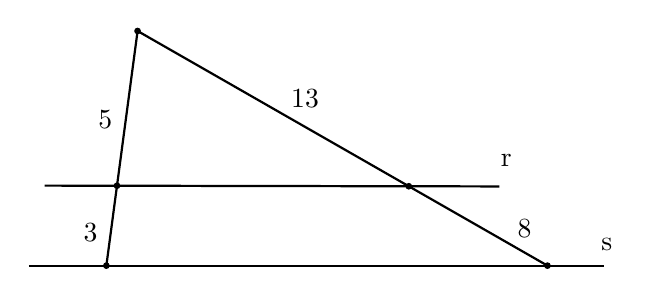
\begin{tikzpicture}
\draw [line width=0.8pt] (-1.,0.)-- (6.307729090909094,0.);
\draw [line width=0.8pt] (0.3818181818181818,2.98)-- (-0.014751470794228672,0.);
\draw [line width=0.8pt] (0.3818181818181818,2.98)-- (5.587090166690014,0.);
\draw [line width=0.8pt] (-0.8,1.0163636363636355)-- (4.976729090909093,1.006014545454545);
\draw (-0.24079090909090867,2.0974345454545427) node[anchor=north west] {5};
\draw (-0.4271309090909089,0.6599545454545442) node[anchor=north west] {3};
\draw (2.2082490909090944,2.3636345454545427) node[anchor=north west] {13};
\draw (5.083209090909098,0.7131945454545442) node[anchor=north west] {8};
\draw (4.870249090909097,1.5384145454545435) node[anchor=north west] {r};
\draw (6.148009090909099,0.47361454545454446) node[anchor=north west] {s};
\draw [fill=black] (-0.014751470794228672,0.) circle (1.0pt);
\draw [fill=black] (5.587090166690014,0.) circle (1.0pt);
\draw [fill=black] (0.3818181818181818,2.98) circle (1.0pt);
\draw [fill=black] (0.12028381420322001,1.014714935047463) circle (1.0pt);
\draw [fill=black] (3.8262485808239415,1.0080756473689043) circle (1.0pt);
\end{tikzpicture}\end{center}\begin{enumerate}
\item {} 
As retas r e s são paralelas?

\item {} 
Justifique sua resposta.

\end{enumerate}

\paragraph{Parte 2} 
Observe a figura a seguir:

\begin{center}
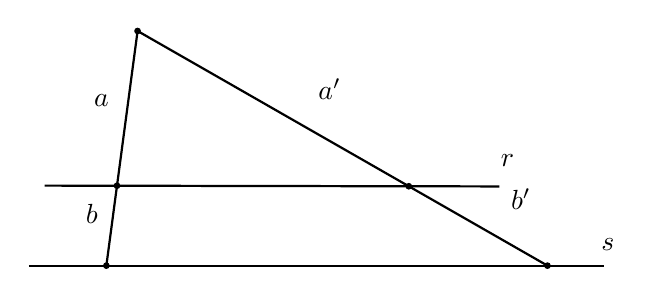
\begin{tikzpicture}
\draw [line width=0.8pt] (-1.,0.)-- (6.307729090909094,0.);
\draw [line width=0.8pt] (0.3818181818181818,2.98)-- (-0.014751470794228672,0.);
\draw [line width=0.8pt] (0.3818181818181818,2.98)-- (5.587090166690014,0.);
\draw [line width=0.8pt] (-0.8,1.0163636363636355)-- (4.976729090909093,1.006014545454545);
\draw (4.870249090909097,1.538414545454544) node[anchor=north west] {$r$};
\draw (6.148009090909099,0.4736145454545451) node[anchor=north west] {$s$};
\draw (-0.29403090909090873,2.3) node[anchor=north west] {$ a $};
\draw (-0.40051090909090886,.9) node[anchor=north west] {$ b $};
\draw (2.554309090909095,2.5) node[anchor=north west] {$ a' $};
\draw (5.0,1.1) node[anchor=north west] {$ b' $};
\draw [fill=black] (-0.014751470794228672,0.) circle (1.0pt);
\draw [fill=black] (5.587090166690014,0.) circle (1.0pt);
\draw [fill=black] (0.3818181818181818,2.98) circle (1.0pt);
\draw [fill=black] (0.12028381420322001,1.014714935047463) circle (1.0pt);
\draw [fill=black] (3.8262485808239415,1.0080756473689043) circle (1.0pt);
\end{tikzpicture}
\end{center}
Na figura acima, se $\frac{a}{a'}=\frac{b}{b'}$ as retas $r$ e $s$ são paralelas? A resposta é sim e essa ideia é a recíproca do teorema de Tales. Você vai agora acompanhar a justificativa desse fato.

\textit{Demonstração}: Consideremos a mesma figura anterior com algumas letras novas

\begin{center}
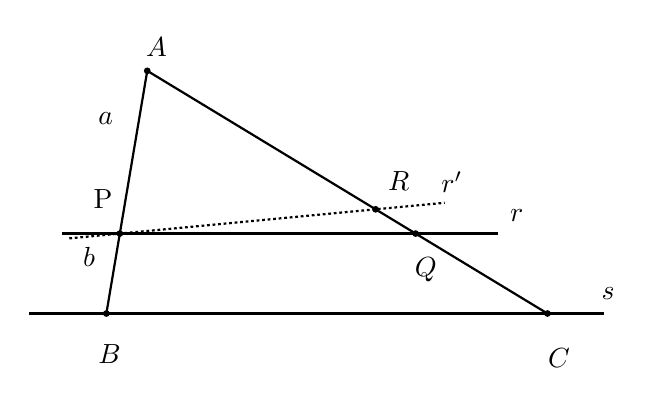
\begin{tikzpicture}
   \draw [line width=0.8pt] (-1.,0.)-- (6.307729090909094,0.);
   \draw [line width=0.8pt] (0.5045690909090926,3.0823745454545417)-- (-0.014751470794228672,0.);
   \draw [line width=0.8pt] (0.5045690909090926,3.0823745454545417)-- (5.587090166690014,0.);
   \draw (4.116661090909101,1.929244545454541) node[anchor=north west] {$r'$};
   \draw (6.149461090909105,0.45304454545454115) node[anchor=north west] {$s$};
   \draw (-0.23933890909090766,2.6794445454545412) node[anchor=north west] {$ a $};
   \draw (-0.43293890909090804,0.9612445454545412) node[anchor=north west] {$ b $};
   \draw (0.36566109090909354,3.623244545454541) node[anchor=north west] {$A$};
   \draw (-0.3,1.7) node[anchor=north west] {P};
   \draw (-0.23933890909090766,-0.27295545454545883) node[anchor=north west] {$B$};
   \draw (5.471861090909104,-0.32135545454545883) node[anchor=north west] {$C$};
   \draw [line width=0.8pt,dash pattern=on 1pt off 1pt] (-0.48558165509078804,0.9544832953920732)-- (4.2819641805126425,1.4065858531455069);
   \draw [line width=0.8pt] (-0.5781389090909086,1.015353941507814)-- (4.963661090909102,1.015353941507814);
   \draw (3.4390610909091,1.929244545454541) node[anchor=north west] {$R$};
   \draw (3.7778610909091004,0.8402445454545412) node[anchor=north west] {$Q$};
   \draw (4.987861090909103,1.445244545454541) node[anchor=north west] {$r$};
   \draw [fill=black] (-0.014751470794228672,0.) circle (1.0pt);
   \draw [fill=black] (5.587090166690014,0.) circle (1.0pt);
   \draw [fill=black] (0.5045690909090926,3.0823745454545417) circle (1.0pt);
   \draw [fill=black] (0.15631605245958863,1.015353941507814) circle (1.0pt);
   \draw [fill=black] (3.404912635547542,1.3234157567409413) circle (1.0pt);
   \draw [fill=black] (3.9128751318232196,1.015353941507814) circle (1.0pt);
\end{tikzpicture}
\end{center}

Por hipótese temos que $\frac{a}{a'}=\frac{b}{b'}$, o que é o mesmo que $\frac{a}{b}=\frac{a'}{b'}$. A primeira fração é a razão em que $P$ divide o segmento $AB$ e a segunda é a razão em que $Q$ divide o segmento $AC$. Elas são iguais, ou seja, $\frac{PA}{PB}=\frac{QA}{QC}$.

Vamos usar agora uma técnica nova de demonstração conhecida como “redução ao absurdo”. Ela consiste em negar a tese, reunir com a hipótese e depois mostrar, com argumentos sólidos, que o que afirmamos não é possível.

Queremos mostrar que as retas $r$ e $s$ são paralelas. Continuando com nossa hipótese, vamos então imaginar o seguinte:

\textit{"Suponha que as retas $r$ e $s$ não são paralelas"}

Bem, dessa forma, vamos traçar agora pelo ponto $P$ uma reta $r'$ paralela à reta $s$. Essa nova reta vai cortar o segmento $AC$ no ponto $R$.

Pelo teorema de Tales, ou melhor, pelo fato de que a projeção paralela conserva as razões, temos que $\frac{PA}{PB}=\frac{RA}{RC}$.

Assim, $\frac{QA}{QC}=\frac{RA}{RC}$ e, portanto, os pontos $Q$ e $R$ devem coincidir.

Como \(\dfrac{QA}{QC}=\dfrac{RA}{RC}\), os pontos \(Q\) e \(R\) coincidem, assim como as retas \(r\) e \(r’\).

\end{task}


\subsection{Demonstração do teorema de Tales usando Áreas}


\paragraph{Duas propriedades dos triângulos:}

A figura a seguir mostra as situações que nos permitirão concluir duas propriedades sobre os triângulos relacionadas às suas áreas.
\begin{center}
\scalebox{1.15}
{
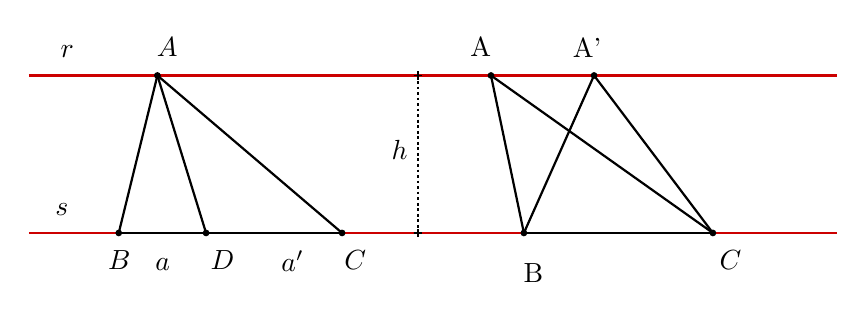
\begin{tikzpicture}
\definecolor{ccqqqq}{rgb}{0.8,0.,0.}
\draw [line width=0.8pt,color=ccqqqq,domain=-4.384390243902435:5.875121951219508] plot(\x,{(-0.-0.*\x)/1.});
\draw [line width=0.8pt,color=ccqqqq,domain=-4.384390243902435:5.875121951219508] plot(\x,{(--2.-0.*\x)/1.});
\draw [line width=0.8pt,dash pattern=on 1pt off 1pt] (0.5581818181818191,2.)-- (0.5581818181818191,0.);
\draw [line width=0.8pt] (-2.7509090909090905,2.)-- (-3.2418181818181813,0.);
\draw [line width=0.8pt] (-3.2418181818181813,0.)-- (-0.4054545454545447,0.);
\draw [line width=0.8pt] (-0.4054545454545447,0.)-- (-2.7509090909090905,2.);]
\draw [line width=0.8pt] (-2.7509090909090905,2.)-- (-2.1327272727272724,0.);
\draw [line width=0.8pt] (1.4854545454545465,2.)-- (1.9036363636363647,0.);
\draw [line width=0.8pt] (1.9036363636363647,0.)-- (4.3036363636363655,0.);
\draw [line width=0.8pt] (4.3036363636363655,0.)-- (1.4854545454545465,2.);
\draw [line width=0.8pt] (2.7945454545454558,2.)-- (1.9036363636363647,0.);
\draw [line width=0.8pt] (2.7945454545454558,2.)-- (4.3036363636363655,0.);
\draw (-2.881951219512193,2.6) node[anchor=north west] {$A$};
\draw (-3.5,-0.1) node[anchor=north west] {$B$};
\draw (-0.5,-0.1) node[anchor=north west] {$C$};
\draw (-2.9,-0.2) node[anchor=north west] {$ a $};
\draw (-2.2,-0.1) node[anchor=north west] {$D$};
\draw (-1.3,-.1) node[anchor=north west] {$ a' $};
\draw (0.1,1.3) node[anchor=north west] {$  h$};
\draw (1.1,2.6) node[anchor=north west] {A};
\draw (1.7756097560975592,-0.25929046563192587) node[anchor=north west] {B};
\draw (4.265365853658532,-0.1) node[anchor=north west] {$C$};
\draw (2.4,2.6) node[anchor=north west] {A'};
\draw (-4.105365853658533,2.5) node[anchor=north west] {$ r$};
\draw (-4.169756097560972,0.5) node[anchor=north west] {$s$};
\draw [fill=black] (-2.7509090909090905,2.) circle (1.0pt);
\draw [fill=black] (-3.2418181818181813,0.) circle (1.0pt);
\draw [fill=black] (-0.4054545454545447,0.) circle (1.0pt);\draw [fill=black] (-2.1327272727272724,0.) circle (1.0pt);
\draw [fill=black] (1.9036363636363647,0.) circle (1.0pt);
\draw [fill=black] (4.3036363636363655,0.) circle (1.0pt);
\draw [fill=black] (1.4854545454545465,2.) circle (1.0pt);
\draw [fill=black] (2.7945454545454558,2.) circle (1.0pt);
\draw [color=black] (0.5581818181818191,2.)-- ++(-1.5pt,0 pt) -- ++(3.0pt,0 pt) ++(-1.5pt,-1.5pt) -- ++(0 pt,3.0pt);
\draw [color=black] (0.5581818181818191,0.)-- ++(-1.5pt,0 pt) -- ++(3.0pt,0 pt) ++(-1.5pt,-1.5pt) -- ++(0 pt,3.0pt);
\end{tikzpicture}
}
\end{center}
Nesta seção, usaremos a notação \((XYZ)\) para denotar a área do triângulo cujos vértices são \(X\), \(Y\) e \(Z\).

A figura mostra as paralelas \(r\) e \(s\) que estão a uma distância \(h\) entre si. Do lado esquerdo aparece o triângulo \(ABC\) dividido em duas partes pelo segmento \(AD\). A primeira propriedade diz respeito aos dois triângulos colados ABD e ADC.

\begin{observationtitle}{Propriedade 1}

\textit{Se dois triângulos possuem mesma altura então a razão entre suas áreas é a razão entre suas bases}.
\end{observationtitle}

De fato, a propriedade pode ser verificada calculando diretamente as áreas dos triângulos \(ABD\) e \(ADC\):
\begin{equation*}
\begin{split}\dfrac{(ABD)}{(ADC)}=\dfrac{\dfrac{a\cdot h}{2}}{\dfrac{a'\cdot h}{2}}=\dfrac{a}{a'}\end{split}
\end{equation*}
Do lado direito da figura acima aparecem os triângulos \(ABC\) e \(A'BC\) que mostram a segunda propriedade.

\begin{observationtitle}{Propriedade 2}

\textit{Dois triângulos de mesma base e mesma altura possuem mesma área}.
\end{observationtitle}

Uma vez que a área do triângulo depende apenas da base e da altura, a propriedade fica bastante evidente. Por outro lado, a interpretação que se dá à propriedade é que, se escolhemos um lado de um triângulo qualquer como base e movemos o terceiro vértice sobre uma paralela à base, o novo triângulo formado tem a mesma área do triângulo original.


\paragraph{Demonstrando o teorema}

Na primeira demonstração do Teorema de Tales, nossa estratégia envolvia o fato de que os segmentos determinados pelas paralelas sobre uma das transversais eram comensuráveis. Nossa nova estratégia não depende dessa condição e, por isso é válida também nos casos em que os segmentos citados não são comensuráveis.

A Hipótese do teorema diz que há um feixe de retas paralelas cortadas por duas trasnversais. Nada é dito sobre as posições das retas transversais e isso significa, em Matemática, que o teorema deve ser válido independentemente dessas posições. Além disso, como visto na demonstração do caso de segmentos comensuráveis, podemos fazer nossa demonstração, sem perder a generalidade do teorema, com um feixe de três retas paralelas, pois essa demonstração pode ser repetida para cada escolha de três retas paralelas do feixe.

O caso trivial do teorema ocorre quando as retas trasnversais são também paralelas, como na figura a seguir:
\begin{center}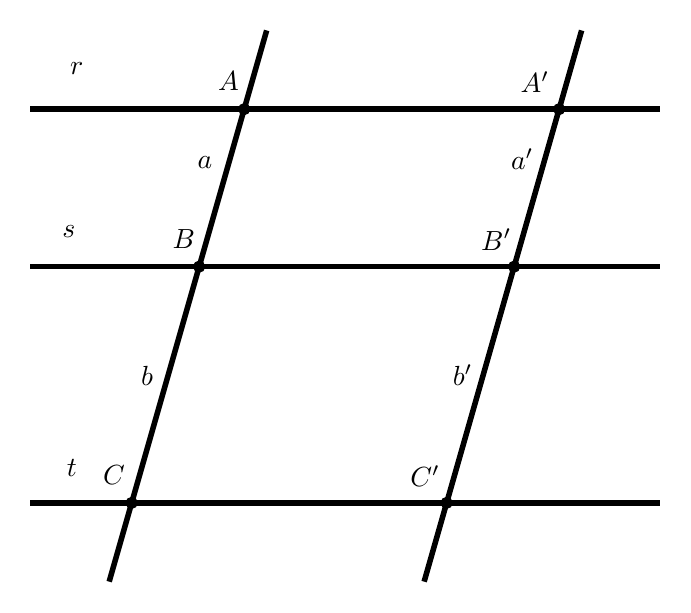
\begin{tikzpicture}
\draw [line width=2.pt] (0.,5.)-- (8.,5.);
\draw [line width=2.pt] (0.,3.)-- (8.,3.);
\draw [line width=2.pt] (0.,0.)-- (8.,0.);
\draw (2.,4.52) node[anchor=north west] {$a$};
\draw (1.28,1.86) node[anchor=north west] {$b$};
\draw (5.98,4.62) node[anchor=north west] {$a'$};
\draw (5.24,1.88) node[anchor=north west] {$b'$};
\draw [line width=2.pt] (3.,6.)-- (1.,-1.);
\draw [line width=2.pt] (7.,6.)-- (5.,-1.);
\draw (0.38,5.72) node[anchor=north west] {$r$};
\draw (0.28,3.64) node[anchor=north west] {$s$};
\draw (0.34,0.68) node[anchor=north west] {$t$};
\draw (2.26,5.6) node[anchor=north west] {$A$};
\draw (1.68,3.6) node[anchor=north west] {$B$};
\draw (0.8,0.6) node[anchor=north west] {$C$};
\draw (6.1,5.6) node[anchor=north west] {$A'$};
\draw (5.6,3.6) node[anchor=north west] {$B'$};
\draw (4.7,0.6) node[anchor=north west] {$C'$};
\draw [fill=black] (2.7142857142857144,5.) circle (2.0pt);
\draw [fill=black] (2.142857142857143,3.) circle (2.0pt);
\draw [fill=black] (1.2857142857142858,0.) circle (2.0pt);
\draw [fill=black] (6.714285714285714,5.) circle (2.0pt);
\draw [fill=black] (6.142857142857143,3.) circle (2.0pt);
\draw [fill=black] (5.285714285714286,0.) circle (2.0pt);
\end{tikzpicture}\end{center}
Nesse caso, \(ABB'A'\) e \(BCC'B'\) são paralelogramos e, por isso, \(a=a'\) e \(b=b'\). Portanto a tese \(\dfrac{a}{b}=\dfrac{a'}{b'}\) é verdadeira.

No caso em que as retas transversais não são paralelas, podemos reduzir a figura a uma mais simples, usando o caso trivial, conforme a figura a seguir:
\begin{center}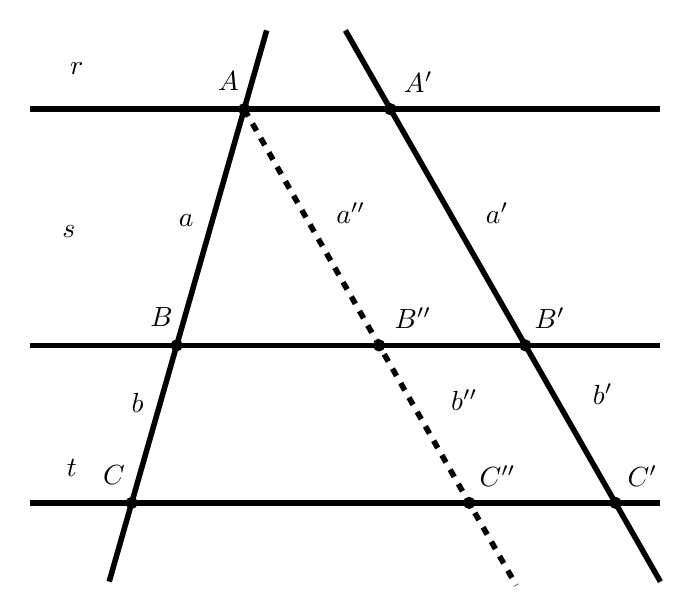
\begin{tikzpicture}
\draw [line width=2.pt] (0.,5.)-- (8.,5.);
\draw [line width=2.pt] (0.,2.)-- (8.,2.);
\draw [line width=2.pt] (0.,0.)-- (8.,0.);
\draw (1.76,3.78) node[anchor=north west] {$a$};
\draw (1.16,1.52) node[anchor=north west] {$b$};
\draw (5.66,3.94) node[anchor=north west] {$a'$};
\draw (7.02,1.64) node[anchor=north west] {$b'$};
\draw [line width=2.pt] (3.,6.)-- (1.,-1.);
\draw (0.38,5.72) node[anchor=north west] {$r$};
\draw (0.28,3.64) node[anchor=north west] {$s$};
\draw (0.34,0.68) node[anchor=north west] {$t$};
\draw (2.26,5.6) node[anchor=north west] {$A$};
\draw (1.4,2.6) node[anchor=north west] {$B$};
\draw (0.8,0.6) node[anchor=north west] {$C$};
\draw (4.62,5.6) node[anchor=north west] {$A'$};
\draw (6.28,2.6) node[anchor=north west] {$B'$};
\draw (7.46,0.6) node[anchor=north west] {$C'$};
\draw [line width=2.pt] (4.,6.)-- (8.,-1.);
\draw [line width=2.pt,dashed] (2.7142857142857144,5.)-- (6.1692307692307695,-1.0461538461538469);
\draw (4.5,2.6) node[anchor=north west] {$B''$};
\draw (5.58,0.6) node[anchor=north west] {$C''$};
\draw (3.76,3.94) node[anchor=north west] {$a''$};
\draw (5.22,1.56) node[anchor=north west] {$b''$};
\draw [fill=black] (2.7142857142857144,5.) circle (2.0pt);
\draw [fill=black] (1.8571428571428572,2.) circle (2.0pt);
\draw [fill=black] (1.2857142857142858,0.) circle (2.0pt);
\draw [fill=black] (4.428571428571429,2.) circle (2.0pt);
\draw [fill=black] (5.571428571428571,0.) circle (2.0pt);
\draw [fill=black] (4.571428571428571,5.) circle (2.0pt);
\draw [fill=black] (6.285714285714286,2.) circle (2.0pt);
\draw [fill=black] (7.428571428571429,0.) circle (2.0pt);
\end{tikzpicture}\end{center}
Como \(a'=a''\) e \(b'=b''\), mostrar que \(\dfrac{a}{b}=\dfrac{a''}{b''}\) mostra também que \(\dfrac{a}{b}=\dfrac{a'}{b'}\), que é a tese de nosso teorema.

Portanto, para mostrar o caso geral, tomemos a figura a seguir, já simplificada, onde as retas \(r\), \(s\) e \(t\) são paralelas e as retas \(OA\) e \(OA'\) são as trasnversais.
\begin{center}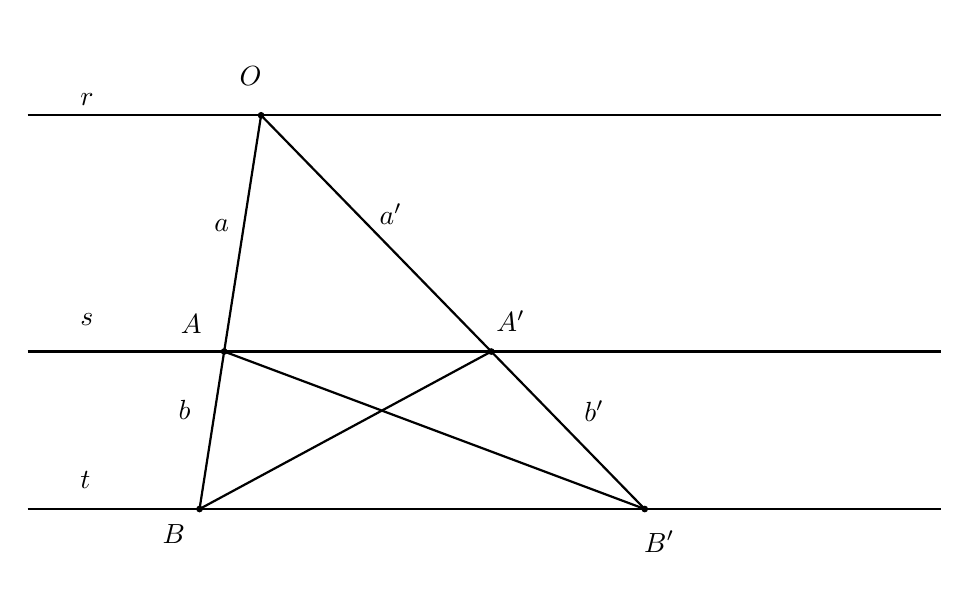
\begin{tikzpicture}
\clip(-6.245361801353108,-0.994413927588976) rectangle (5.35363262685944,6.113077489908864);
\draw [line width=0.8pt,domain=-6.245361801353108:47.35363262685944] plot(\x,{(-0.-0.*\x)/1.});
\draw [line width=0.8pt,domain=-6.245361801353108:47.35363262685944] plot(\x,{(--2.-0.*\x)/1.});
\draw [line width=0.8pt,domain=-6.245361801353108:47.35363262685944] plot(\x,{(--5.-0.*\x)/1.});
\draw [line width=0.8pt] (-3.2809171581007854,5.)-- (-4.062560888816656,0.);
\draw [line width=0.8pt] (-3.2809171581007854,5.)-- (1.5913287633614788,0.);
\draw [line width=0.8pt] (-4.062560888816656,0.)-- (-0.3575696052234269,2.);
\draw [line width=0.8pt] (-3.749903396530308,2.)-- (1.5913287633614788,0.);
\draw (-5.7,5.4) node[anchor=north west] {$r$};
\draw (-5.7,2.6) node[anchor=north west] {$ s $};
\draw (-5.7,.6) node[anchor=north west] {$ t $};
\draw (-4,3.8) node[anchor=north west] {$ a $};
\draw (-4.452437691958675,1.5) node[anchor=north west] {$ b $};
\draw (-1.9,4) node[anchor=north west] {$ a' $};
\draw (0.7,1.5) node[anchor=north west] {$  b'$};
\draw [fill=black] (-3.2809171581007854,5.) circle (1.0pt);
\draw[color=black] (-3.4144289970461084,5.499708715642349) node {$O$};
\draw [fill=black] (-4.062560888816656,0.) circle (1.0pt);
\draw[color=black] (-4.389528074085187,-0.3194309376553625) node {$B$};
\draw [fill=black] (1.5913287633614788,0.) circle (1.0pt);
\draw[color=black] (1.7756144775167264,-0.41379536446559567) node {$B'$};
\draw [fill=black] (-3.749903396530308,2.) circle (1.0pt);
\draw[color=black] (-4.169344411527976,2.3542278219679105) node {$A$};
\draw [fill=black] (-0.3575696052234269,2.) circle (1.0pt);
\draw[color=black] (-0.11167405868794078,2.385682630904655) node {$A'$};
\end{tikzpicture}\end{center}
Com os elementos da figura acima observe inicialmente que os triângulos \(A'AB\) e \(AA'B'\)  possuem mesma área pois têm a mesma base \(AA'\) e mesma altura, pois as retas \(s\) e \(t\) são paralelas (\textbf{Propriedade 2}).

Agora, utilizando a \textbf{Propriedade 1}, temos que
\begin{equation*}
\begin{split}\dfrac{a}{b}=\dfrac{(A'OA)}{(A'AB)}=\dfrac{(AOA')}{(AA´B'}=\dfrac{a'}{b'}\end{split}
\end{equation*}
A igualdade \(\dfrac{a}{b}=\dfrac{a'}{b'}\) é nossa tese, o que encerra a demonstração.


\exercise

\begin{enumerate}
\item {} 
O ponto P divide o segmento \(AB\) na razão \(\frac{PA}{PB}=\frac{3}{7}\).
\begin{enumerate}
\item {} 
Qual a raz00ão \(\frac{AP}{AB}\)?

\item {} 
Se \(M\) é o ponto médio do segmento \(AB\) qual é a razão \(\frac{MP}{MB}\)?

\end{enumerate}

\item {} 
Na figura a seguir, \(PQ\) é paralelo a \(BC\). Se \(AP = 5\), \(PB = 4\) e \(QC = 6\), determine a medida do segmento  \(AQ\).
\begin{center}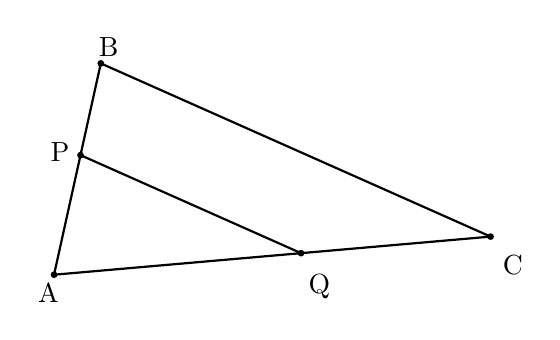
\begin{tikzpicture}
\draw [line width=0.8pt] (-2.632,2.054)-- (2.912,2.538);
\draw [line width=0.8pt] (2.912,2.538)-- (-2.038,4.738);
\draw [line width=0.8pt] (-2.038,4.738)-- (-2.632,2.054);
\draw [line width=0.8pt] (0.5048807378578668,2.327854667590766)-- (-2.2959056352295146,3.572648611185158);
\draw (-2.9598,2.0628) node[anchor=north west] {A};
\draw (-2.1854,5.1846) node[anchor=north west] {B};
\draw (2.945,2.4258) node[anchor=north west] {C};
\draw (-2.8,3.8536) node[anchor=north west] {P};
\draw (0.4766,2.1838) node[anchor=north west] {Q};
\draw [fill=black] (-2.632,2.054) circle (1.0pt);
\draw [fill=black] (2.912,2.538) circle (1.0pt);
\draw [fill=black] (-2.038,4.738) circle (1.0pt);
\draw [fill=black] (0.5048807378578668,2.327854667590766) circle (1.0pt);
\draw [fill=black] (-2.2959056352295146,3.572648611185158) circle (1.0pt);
\end{tikzpicture}\end{center}
\item {} 
Na figura a seguir, \(MN\) é paralelo a \(BC\) e \(NP\) é paralelo a \(AD\). Sabe-se que \(\frac{MA}{MB}=\frac{3}{5}\) e que \(CD = 12\) cm. Quanto mede o segmento \(DP\)?
\begin{center}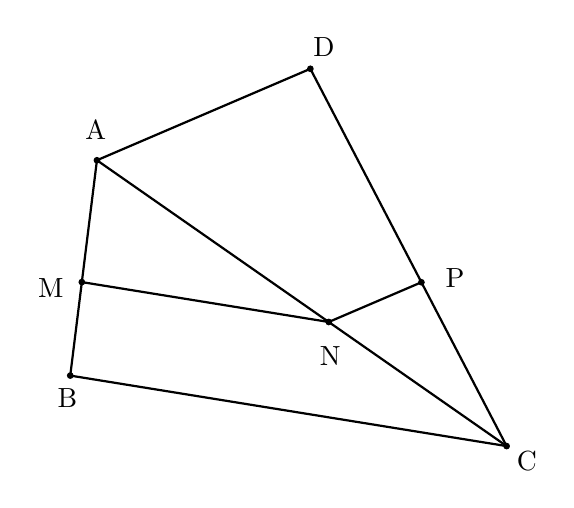
\begin{tikzpicture}
\draw [line width=0.8pt] (-2.4274,3.2728)-- (2.7756,-0.3572);
\draw [line width=0.8pt] (2.7756,-0.3572)-- (-2.7662,0.5382);
\draw [line width=0.8pt] (-2.7662,0.5382)-- (-2.4274,3.2728);
\draw [line width=0.8pt] (0.5165376766007355,1.2188899930692538)-- (-2.619098267313536,1.725521128112171);
\draw (-2.7,3.9) node[anchor=north west] {A};
\draw (-3.04934,0.5) node[anchor=north west] {B};
\draw (2.78044,-0.3) node[anchor=north west] {C};
\draw (1.87536,2.021417999999998) node[anchor=north west] {P};
\draw [line width=0.8pt] (2.7756,-0.3572)-- (0.283,4.4344);
\draw [line width=0.8pt] (-2.4274,3.2728)-- (0.283,4.4344);
\draw [line width=0.8pt] (0.5165376766007355,1.2188899930692538)-- (1.6933515380924455,1.7232387908514153);
\draw (-3.3,1.9) node[anchor=north west] {M};
\draw (0.27816,1.0364779999999998) node[anchor=north west] {N};
\draw (0.1983,4.949617999999992) node[anchor=north west] {D};
\draw [fill=black] (-2.4274,3.2728) circle (1.0pt);
\draw [fill=black] (2.7756,-0.3572) circle (1.0pt);
\draw [fill=black] (-2.7662,0.5382) circle (1.0pt);
\draw [fill=black] (0.5165376766007355,1.2188899930692538) circle (1.0pt);
\draw [fill=black] (-2.619098267313536,1.725521128112171) circle (1.0pt);
\draw [fill=black] (0.283,4.4344) circle (1.0pt);
\draw [fill=black] (1.6933515380924455,1.7232387908514153) circle (1.0pt);
\end{tikzpicture}\end{center}
\item {} 
Na figura a seguir as retas \(r\) e \(s\) são paralelas e os segmentos \(CE\) e \(EG\) são paralelos. Sabe-se que \(AE = 2\), \(EB = 6\) e que o segmento \(ED\) tem 7 unidades a mais que \(CE\).
\begin{enumerate}
\item {} 
Quanto mede o segmento \(CD\)?

\item {} 
Sabe-se que \(FD = 16\). Trace o segmento \(CF\) e trace por \(E\) uma paralela a \(CF\) que encontra a reta \(s\) em \(G\). Quanto mede \(GD\)?

\end{enumerate}
\begin{center}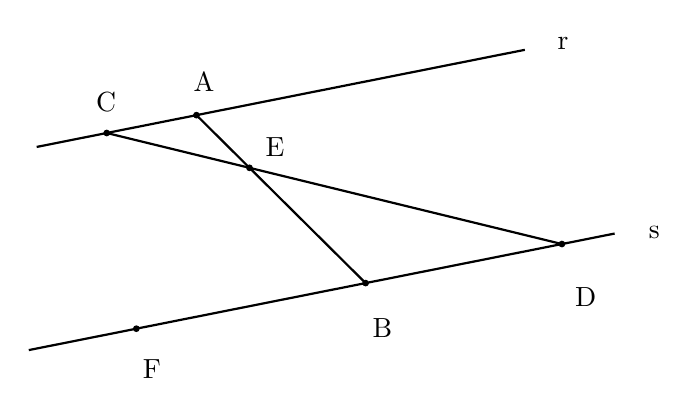
\begin{tikzpicture}
\draw [line width=0.8pt] (-2.64,0.46)-- (4.8,1.94);
\draw [line width=0.8pt] (-2.54,3.04)-- (3.6596296600058285,4.273259663549546);
\draw [line width=0.8pt] (-1.6499582116298486,3.217051323492987)-- (4.130679271513971,1.806855554010844);
\draw [line width=0.8pt] (-0.5106335307872909,3.4436911793595173)-- (1.6378189906853886,1.3109639927707495);
\draw (-0.6721669353242998,4.102723170072155) node[anchor=north west] {A};
\draw (1.602133160970336,0.9879208642773318) node[anchor=north west] {B};
\draw (-1.9081995963539933,3.855516637866216) node[anchor=north west] {C};
\draw (4.1730810959120985,1.3834513158068331) node[anchor=north west] {D};
\draw (0.24249723383767327,3.286941613792558) node[anchor=north west] {E};
\draw (-1.3149039190597405,0.4687871466448614) node[anchor=north west] {F};
\draw (3.9505952169267533,4.547694928042843) node[anchor=north west] {r};
\draw (5.1124659182946655,2.1497915656452418) node[anchor=north west] {s};
\draw [fill=black] (-1.6499582116298486,3.217051323492987) circle (1.0pt);
\draw [fill=black] (4.130679271513971,1.806855554010844) circle (1.0pt);
\draw [fill=black] (-0.5106335307872909,3.4436911793595173) circle (1.0pt);
\draw [fill=black] (1.6378189906853886,1.3109639927707495) circle (1.0pt);
\draw [fill=black] (0.16328175964055147,2.774708529294657) circle (1.0pt);
\draw [fill=black] (-1.2743622966773251,0.7316591130265537) circle (1.0pt);
\end{tikzpicture}\end{center}
\item {} 
No triângulo \(ABC\) seja \(AD\) a bissetriz do ângulo \(\hat{A}\) como na figura a seguir. O teorema da bissetriz afirma que \(\frac{DB}{DC}=\frac{AB}{AC}\).

Prove esse teorema usando a sugestão a seguir.
\begin{itemize}
\item {} 
Trace por \(B\) e \(C\) paralelas à bissetriz.

\item {} 
A reta \(BA\) encontra a paralela traçada por \(C\) em \(E\).

\item {} 
Mostre que o triângulo \(ACE\) é isósceles.

\item {} 
Use o teorema de Tales para concluir o resultado.

\end{itemize}
\begin{center}\begin{tikzpicture}
\draw [shift={(1.24,2.22)},line width=0.8pt,color=session2,fill=session2,fill opacity=0.10000000149011612] (0,0) -- (-145.5816355209438:0.5668898395840698) arc (-145.5816355209438:-98.58725411426902:0.5668898395840698) -- cycle;   \draw [shift={(1.24,2.22)},line width=0.8pt,color=session2,fill=session2,fill opacity=0.10000000149011612] (0,0) -- (-98.58725411426903:0.5668898395840698) arc (-98.58725411426903:-51.59287270759427:0.5668898395840698) -- cycle;
\draw [line width=1.2pt] (1.24,2.22)-- (-2.,0.);
\draw [line width=1.2pt] (-2.,0.)-- (3.,0.);
\draw [line width=1.2pt] (3.,0.)-- (1.24,2.22);
\draw [line width=0.8pt] (1.24,2.22)-- (0.9047617009708229,0.);
\draw [line width=0.8pt,dash pattern=on 2pt off 2pt] (-1.4100628574084908,3.9066552370233936)-- (-2.130083863624808,-0.861435516417351);
\draw [line width=0.8pt,dash pattern=on 2pt off 2pt] (1.5063338058635691,3.983703761561156)-- (1.24,2.22);
\draw [line width=0.8pt,dash pattern=on 2pt off 2pt] (0.9047617009708229,0.)-- (0.77504260134413,-0.8590199926595905);
\draw [line width=0.8pt,dash pattern=on 2pt off 2pt] (3.6123080319008642,4.0547987349786965)-- (2.8770410481896134,-0.814253245555635);
\draw (0.7,2.8) node[anchor=north west] {A};
\draw (-2.6,-0.11250549465400854) node[anchor=north west] {B};
\draw (0.9449278317440784,-0.1691944786124154) node[anchor=north west] {D};
\draw (3.0991092221635435,-0.13140182264014416) node[anchor=north west] {C};
\draw (0.5,1.8) node[anchor=north west] {$\theta$};
\draw (1.2,1.7) node[anchor=north west] {$\theta$};
\draw [fill=black] (-2.,0.) circle (1.0pt);
\draw [fill=black] (3.,0.) circle (1.0pt);
\draw [fill=black] (1.24,2.22) circle (1.0pt);
\draw [fill=black] (0.9047617009708229,0.) circle (1.0pt);
\end{tikzpicture}\end{center}
\item {} 
Invente um triângulo \(ABC\) dando medidas para os seus três lados. A bissetriz do ângulo \(\hat{A}\) encontra o lado \(BC\) no ponto \(D\). Calcule os comprimentos dos segmentos \(BD\) e \(DC\).

\item {} 
No triângulo \(ABC\), \(AB = 9\), \(BC = 10\) e \(AC = 6\). A bissetriz do ângulo \(\hat{A}\) encontra o lado \(BC\) no ponto \(D\) e o ponto \(J\) é o incentro do triângulo. Calcule a razão \(\frac{JA}{JD}\).

\item {} 
(CEFE-MG - 2017) A figura a seguir é um esquema representativo de um eclipse lunar em que a Lua, a Terra e o Sol estão representados pelas circunferências de centros \(C_1\), \(C_2\) e \(C_3\) respectivamente, que se encontram alinhados. Considera-se que a distância entre os centros da Terra e do Sol é 400 vezes a distância entre os centros da Terra e da Lua e que a distância do ponto \(T\)  na superfície da Terra ao ponto \(S\) na superfície do Sol, como representados na figura, é de 150 milhões de quilômetros.
\begin{center}
\scalebox{.75}
{
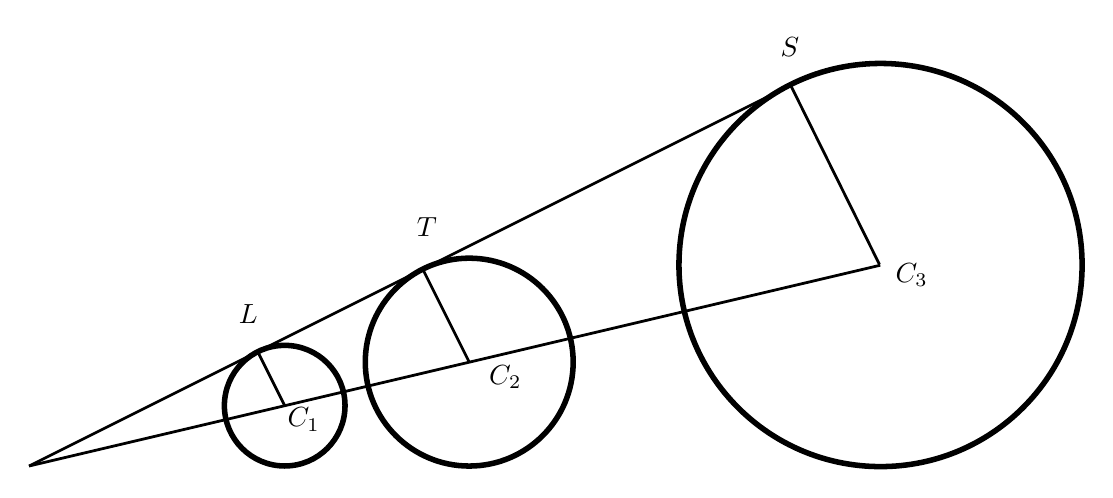
\begin{tikzpicture}
\draw [line width=2.pt] (1.2467707033296944,-1.2335414066593893) circle (0.766);
\draw [line width=2.pt] (3.5901699437494745,-0.6803398874989484) circle (1.32);
\draw [line width=2.pt] (8.813624739188983,0.5527505216220345) circle (2.56);
\draw [line width=1.pt] (-2.,-2.)-- (8.81,0.55);
\draw [line width=1.pt] (8.8,0.56)-- (7.672,2.836);
\draw [line width=1.pt] (3.5901699437494745,-0.6803398874989484)-- (3.,0.5);
\draw [line width=1.pt] (1.2467707033296944,-1.2335414066593893)-- (0.904,-0.548);
\draw [line width=1.pt] (-2.,-2.)-- (7.672,2.836);
\draw (1.16,-1.14) node[anchor=north west] {$C_1$};
\draw (3.72,-0.6) node[anchor=north west] {$C_2$};
\draw (8.88,0.7) node[anchor=north west] {$C_3$};
\draw (0.54,0.18) node[anchor=north west] {$L$};
\draw (2.8,1.28) node[anchor=north west] {$T$};
\draw (7.42,3.56) node[anchor=north west] {$S$};
\end{tikzpicture}
}
\end{center}
Sabendo-se que os segmentos de reta \(C_1L\), \(C_2T\) e \(C_3S\) são paralelos, quanto mede a distância do ponto \(L\)  representado na superfície da Lua, ao ponto \(T\)  na superfície da Terra?

\end{enumerate}


% \ifnum\aluno=1
% \clearpage
% \else
% \notasfinais
% \fi

\bibliographystyle{apalike-pt}
\bibliography{../Bibliografia/probabilidade1_bibliografia.bib}

\nocite{*}
